\documentclass[12pt, a4paper]{article}
\usepackage[english]{babel}
\usepackage[utf8x]{inputenc}
\usepackage[T1]{fontenc}
\usepackage[a4paper]{geometry}
\usepackage{amsmath}
\usepackage{graphicx}
\usepackage[colorlinks=true, allcolors=blue]{hyperref}
\usepackage{epsfig,amsfonts}
\usepackage{natbib}
\usepackage{amssymb}
\usepackage{amsthm}
\usepackage{authblk}
\usepackage{setspace}
\usepackage{hypcap}
\usepackage{xr}
%From: https://tex.stackexchange.com/questions/337/how-to-change-certain-pages-into-landscape-portrait-mode
\usepackage{lscape}

\title{Scrap: Differential complex trait architecture across humans: epistasis identified in non-European populations at multiple genomic scales}
\author[1,2]{Michael C. Turchin}
\author[1,3]{Isabella Ting}
\author[1,4,5,*]{Lorin Crawford}
\author[1,2,*,$\dag$]{Sohini Ramachandran}
\affil[1]{Center for Computational Molecular Biology, Brown University}
\affil[2]{Department of Ecology and Evolutionary Biology, Brown University}
\affil[3]{Department of Computer Science, Brown University}
\affil[4]{Department of Biostatistics, Brown University}
\affil[5]{Center for Statistical Science, Brown University}
\affil[$\ast$]{indicates these authors contributed equally}
\affil[$^\dag$]{To whom correspondence should be addressed: sramachandran@brown.edu}

\begin{document}

\maketitle

%1.17. Contribution to the Field Statement
%When you submit your manuscript, you will be required to briefly summarize in 200 words your manuscript’s contribution to, and position in, the existing literature in your field. This should be written avoiding any technical language or non-standard acronyms. The aim should be to convey the meaning and importance of this research to a non-expert. While Frontiers evaluates articles using objective criteria, rather than impact or novelty, your statement should frame the question(s) you have addressed in your work in the context of the current body of knowledge, providing evidence that the findings—whether positive or negative—contribute to progress in your research discipline. This will assist the Chief Editors to determine whether your manuscript fits within the scope of a specialty as defined in its mission statement; a detailed statement will also facilitate the identification of the editors and reviewers most appropriate to evaluate your work, ultimately expediting your manuscript's initial consideration.

%Example Statement on: Markram K and Markram H (2010) The Intense World Theory – a unifying theory of the neurobiology of autism. Front. Hum. Neurosci. 4:224. doi: 10.3389/fnhum.2010.00224

%Autism spectrum disorders are a group of neurodevelopmental disorders that affect up to 1 in 100 individuals. People with autism display an array of symptoms encompassing emotional processing, sociability, perception and memory, and present as uniquely as the individual. No theory has suggested a single underlying neuropathology to account for these diverse symptoms. The Intense World Theory, proposed here, describes a unifying pathology producing the wide spectrum of manifestations observed in autists. This theory focuses on the neocortex, fundamental for higher cognitive functions, and the limbic system, key for processing emotions and social signals. Drawing on discoveries in animal models and neuroimaging studies in individuals with autism, we propose how a combination of genetics, toxin exposure and/or environmental stress could produce hyper-reactivity and hyper-plasticity in the microcircuits involved with perception, attention, memory and emotionality. These hyper-functioning circuits will eventually come to dominate their neighbors, leading to hyper-sensitivity to incoming stimuli, over-specialization in tasks and a hyper-preference syndrome. We make the case that this theory of enhanced brain function in autism explains many of the varied past results and resolves conflicting findings and views and makes some testable experimental predictions.

\section{Contribution to the Field Statement}\label{Contribution-Field}



\section{Scrap}\label{Supplementary-Figures}

%\begin{figure}[htbp]
%\centering
%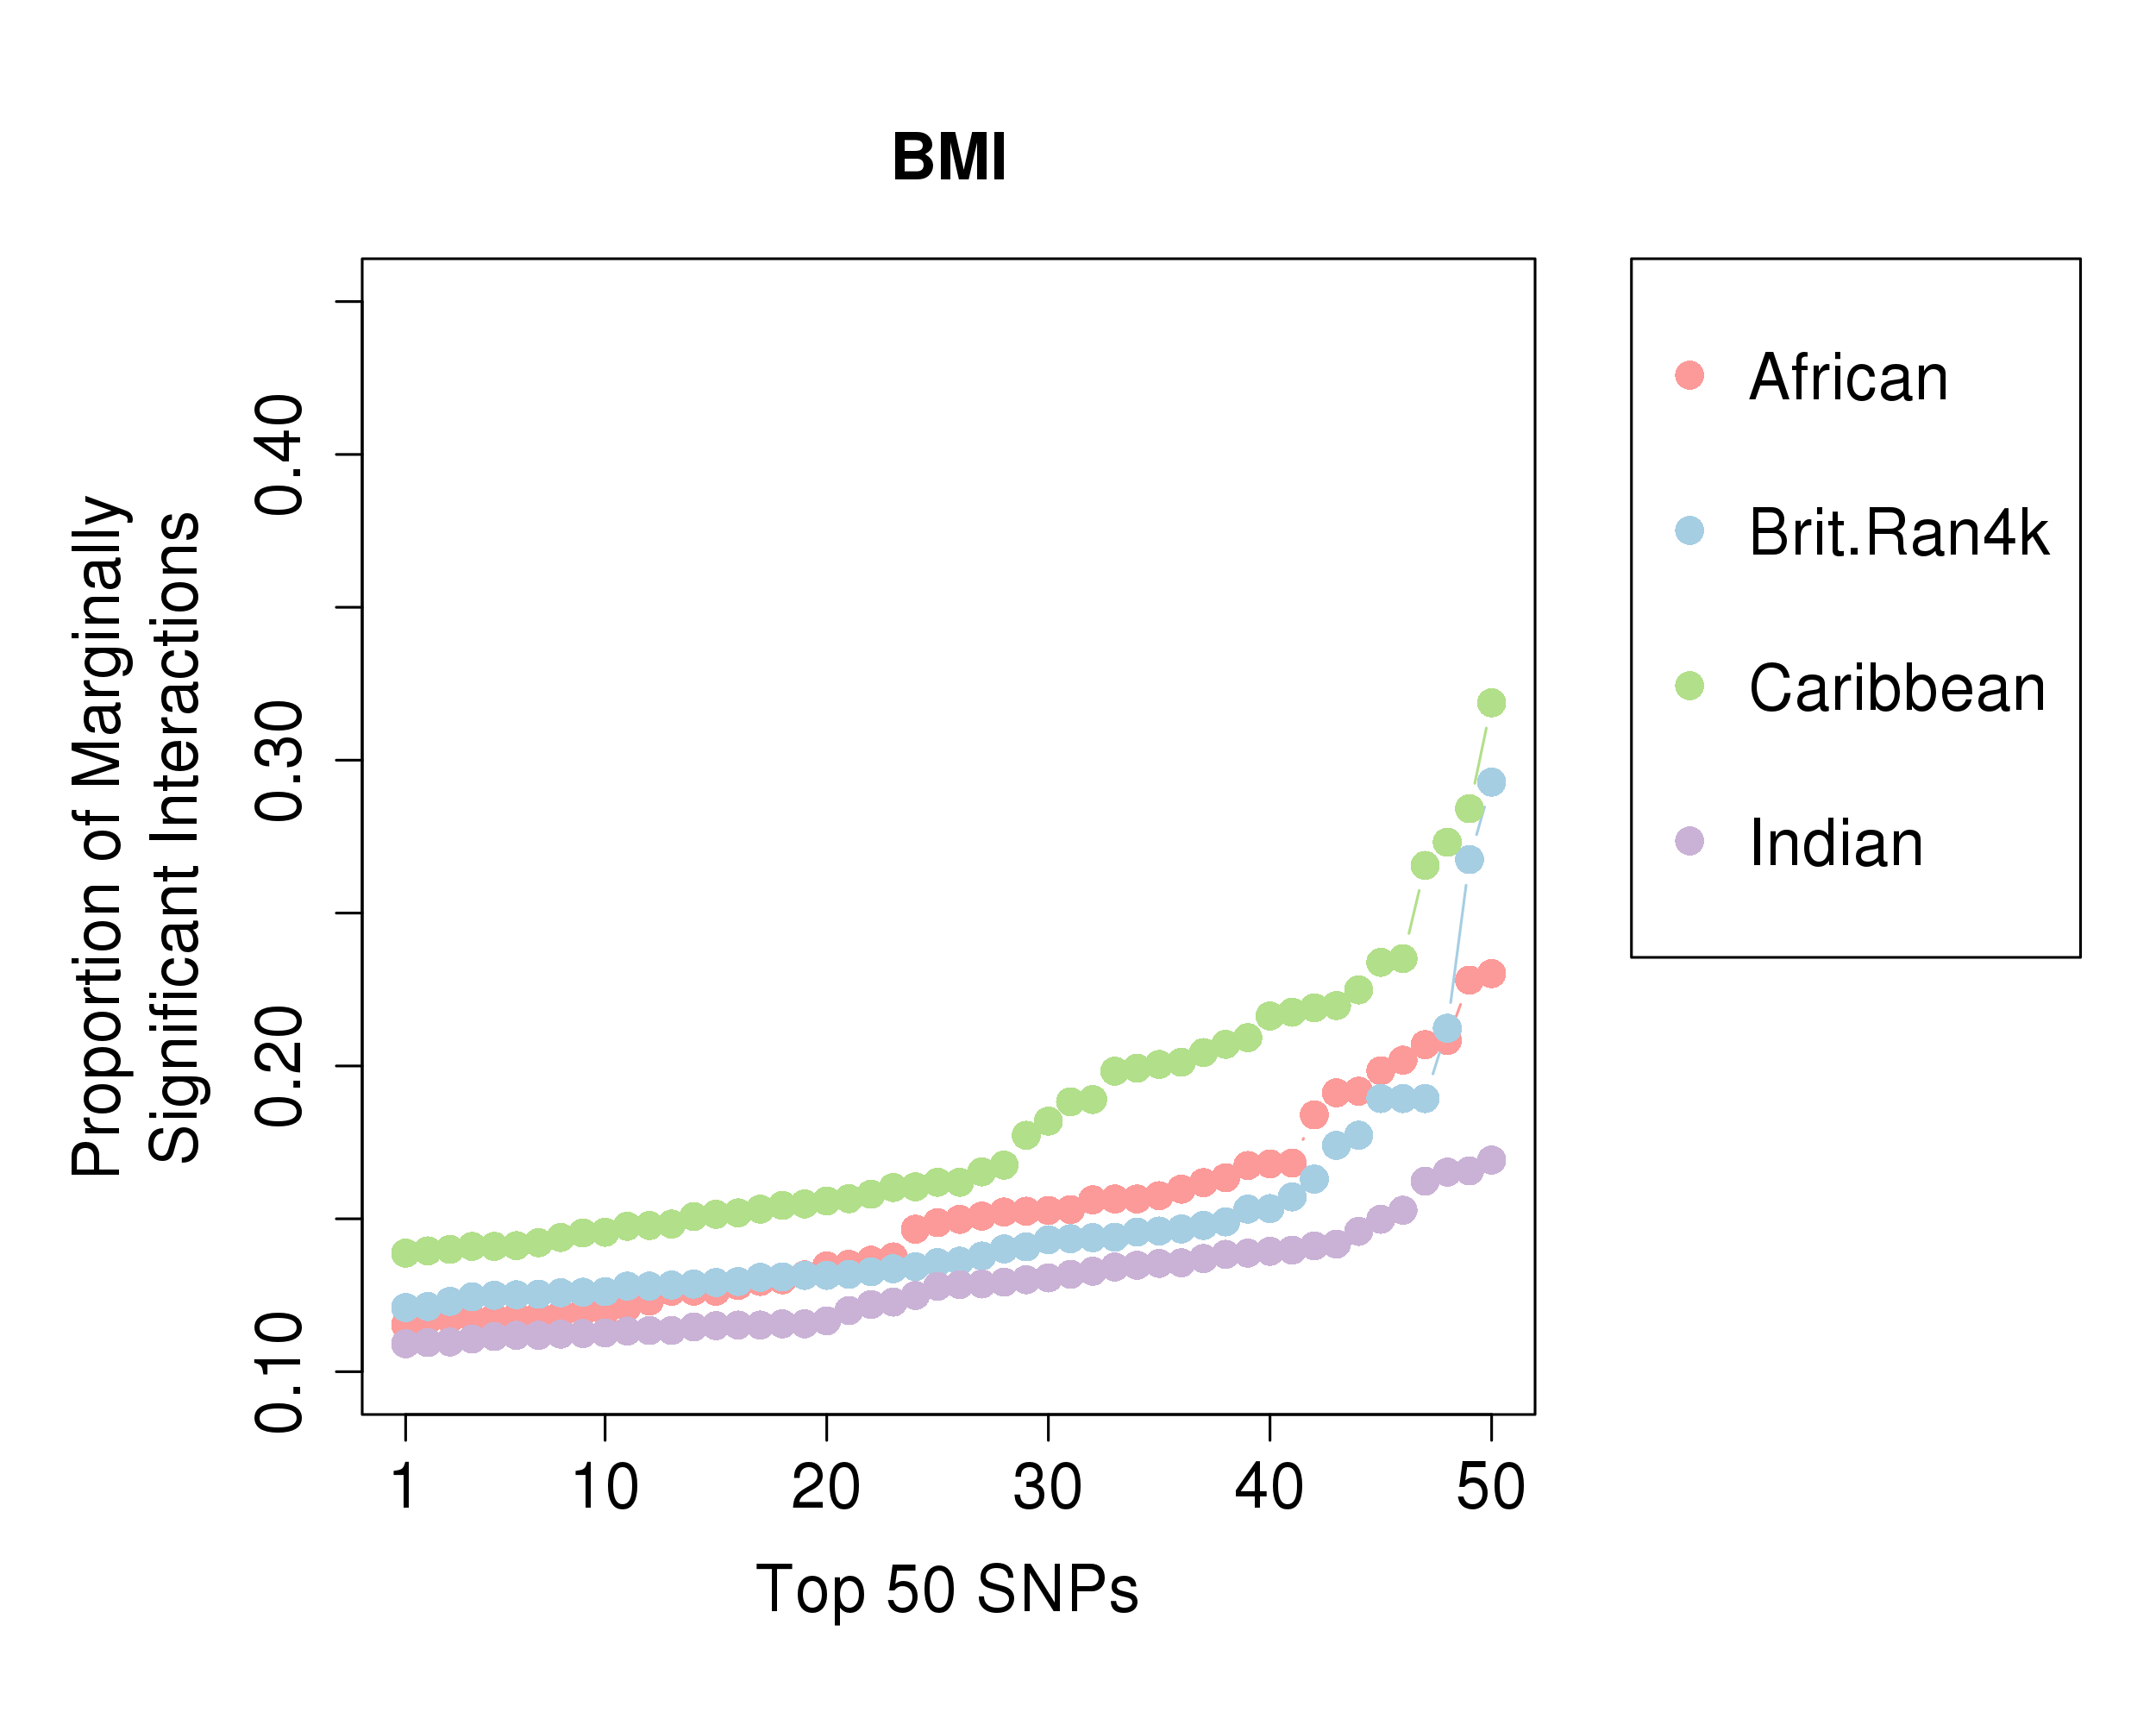
\includegraphics[scale=.5]{Images/Supp/InterPath_Supp_Figure_PLINK_vs3_BMI.png}
%\caption[TBD]{\textbf{PLINK Epistasis Proportion Results: BMI}. The figure shows the proportion of pairwise marginally significant epistatic interactions a single SNP contains when tested on height within our UKB subgroups. Pairwise tests are conducted exhaustively for each individual SNP through PLINK. Marginally significant is defined as pairwise SNP epistasis $p$-value $< 1\times10^{-4}$. Only the top 50 SNPs sorted by decreasing proportion are shown for each UKB subgroup. For results on height see Figure \ref{InterPath-Main-Figure-PLINK-Proportions-Height}. In general we find that the African and Caribbean subgroups have the highest proportions of marginally significant interactions per SNP.}
%\label{InterPath-Supp-Figure-PLINK-Proportions-BMI}
%\end{figure}

%\begin{figure}[htb]
%\centering
%\hspace*{-1.7cm}
%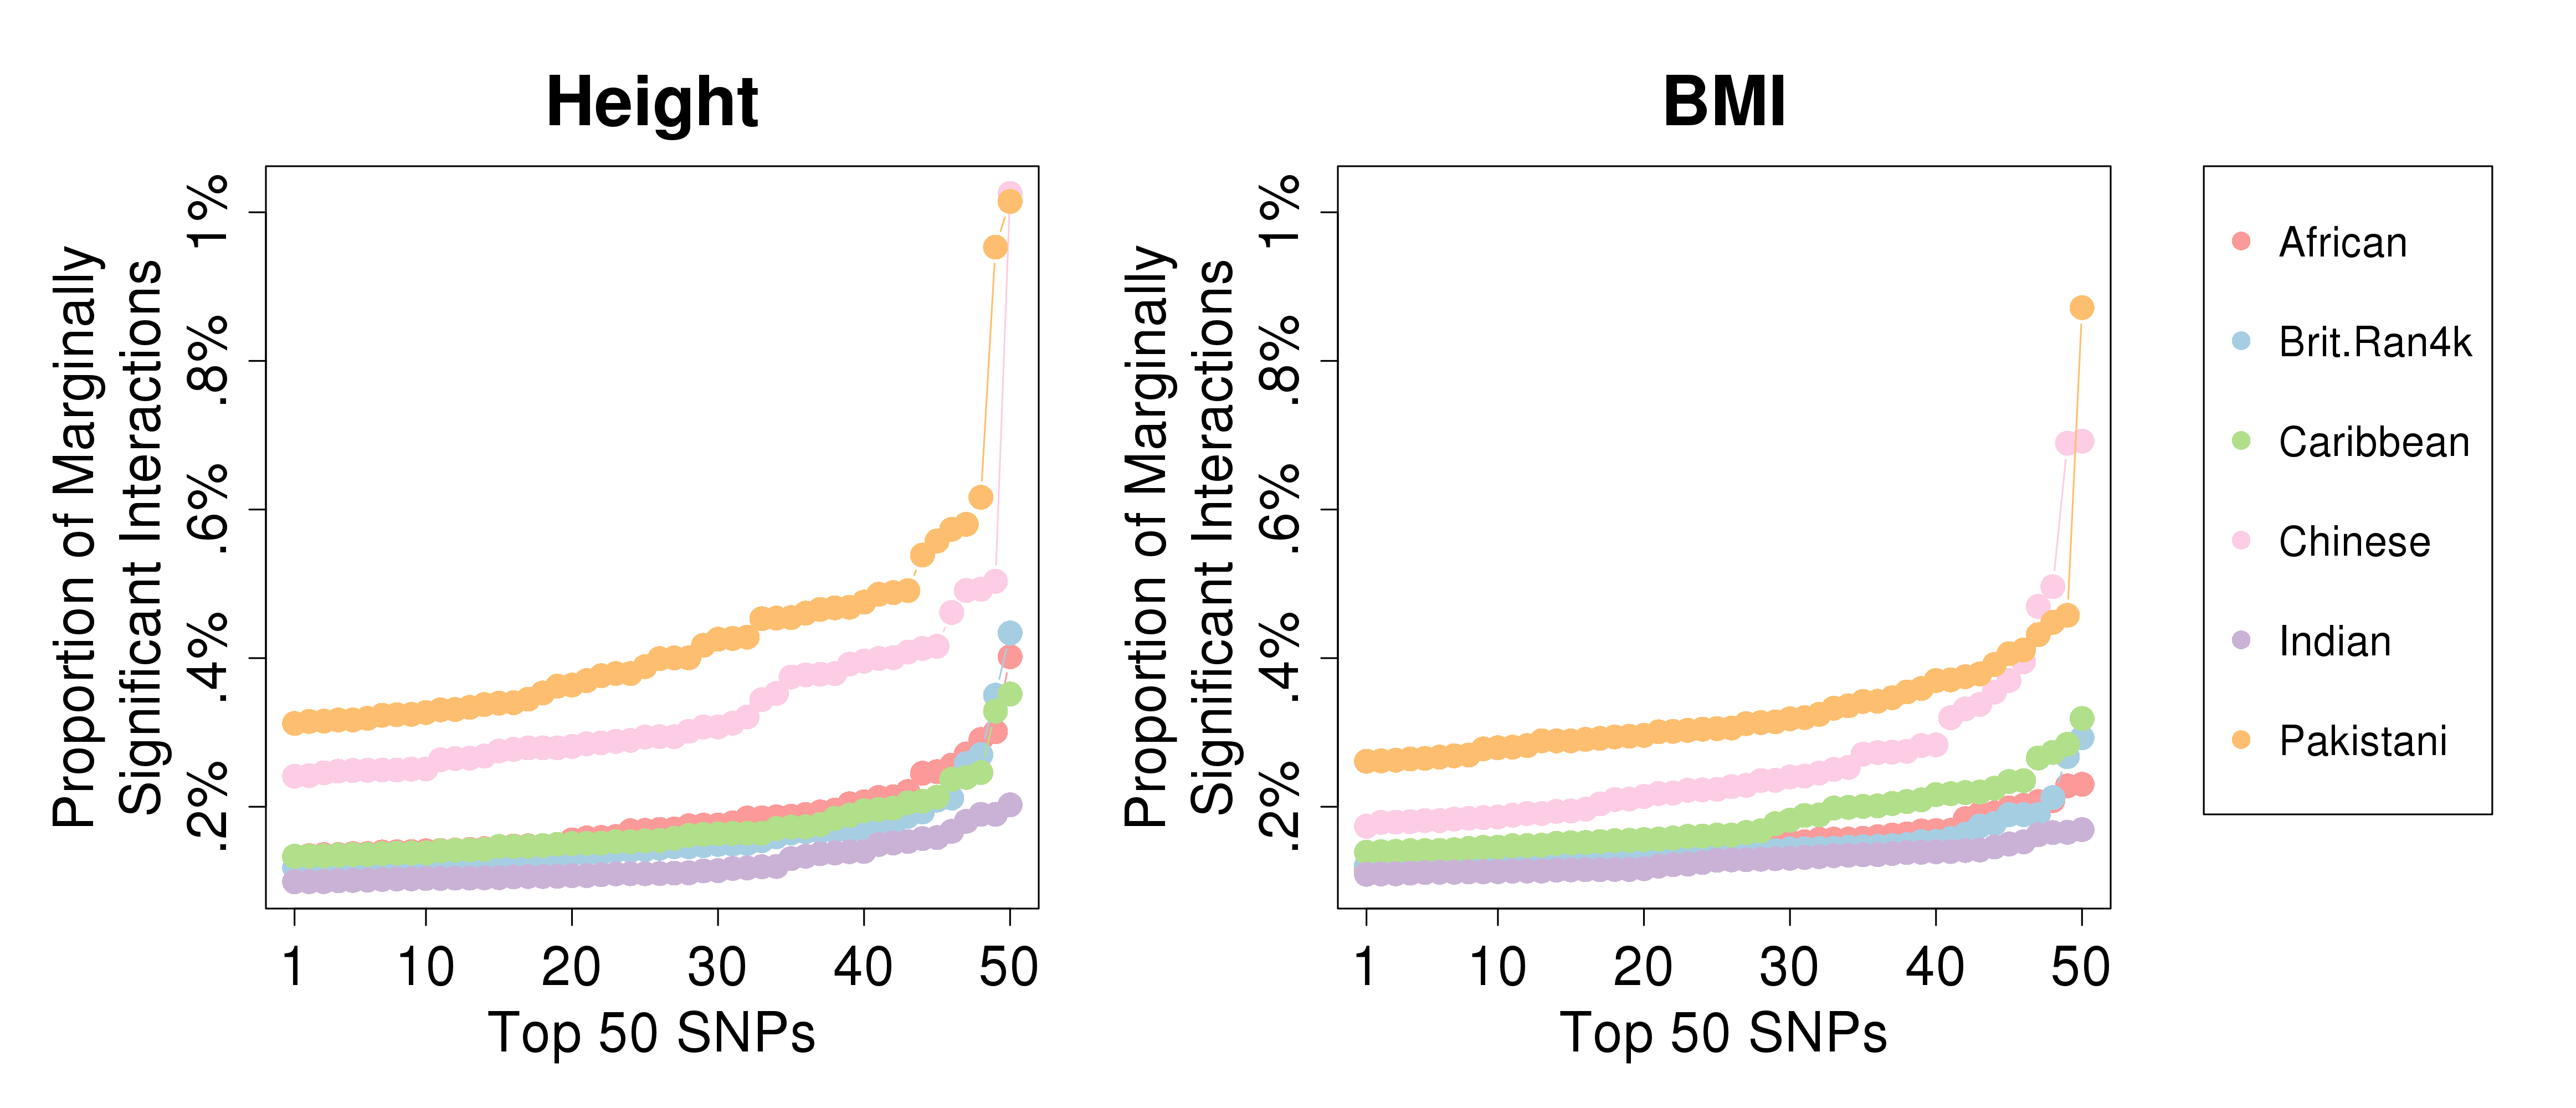
\includegraphics[scale=.45]{Images/Main/InterPath_Main_Figure_PLINK_vs4_HeightBMI.png}
%\caption[TBD]{\textbf{SNPs with the largest proportions of marginally significant PLINK pairwise epistasis tests, per subgroup}. The figure shows the proportion of pairwise marginally significant epistatic interactions a single SNP contains when tested on height and BMI within our UKB subgroups. Pairwise tests are conducted exhaustively for each individual SNP through PLINK. Marginally significant is defined as a pairwise SNP epistasis $p$-value $< 1\times10^{-4}$. Only the top 50 SNPs sorted by decreasing proportion are shown for each UKB subgroup. In general we find that the African and Caribbean subgroups have the highest proportions of marginally significant interactions per SNP.}
%\label{InterPath-Supp-Figure-PLINK-Proportions-HeightBMI}
%\end{figure}

%\begin{figure}[htbp]
%\centering
%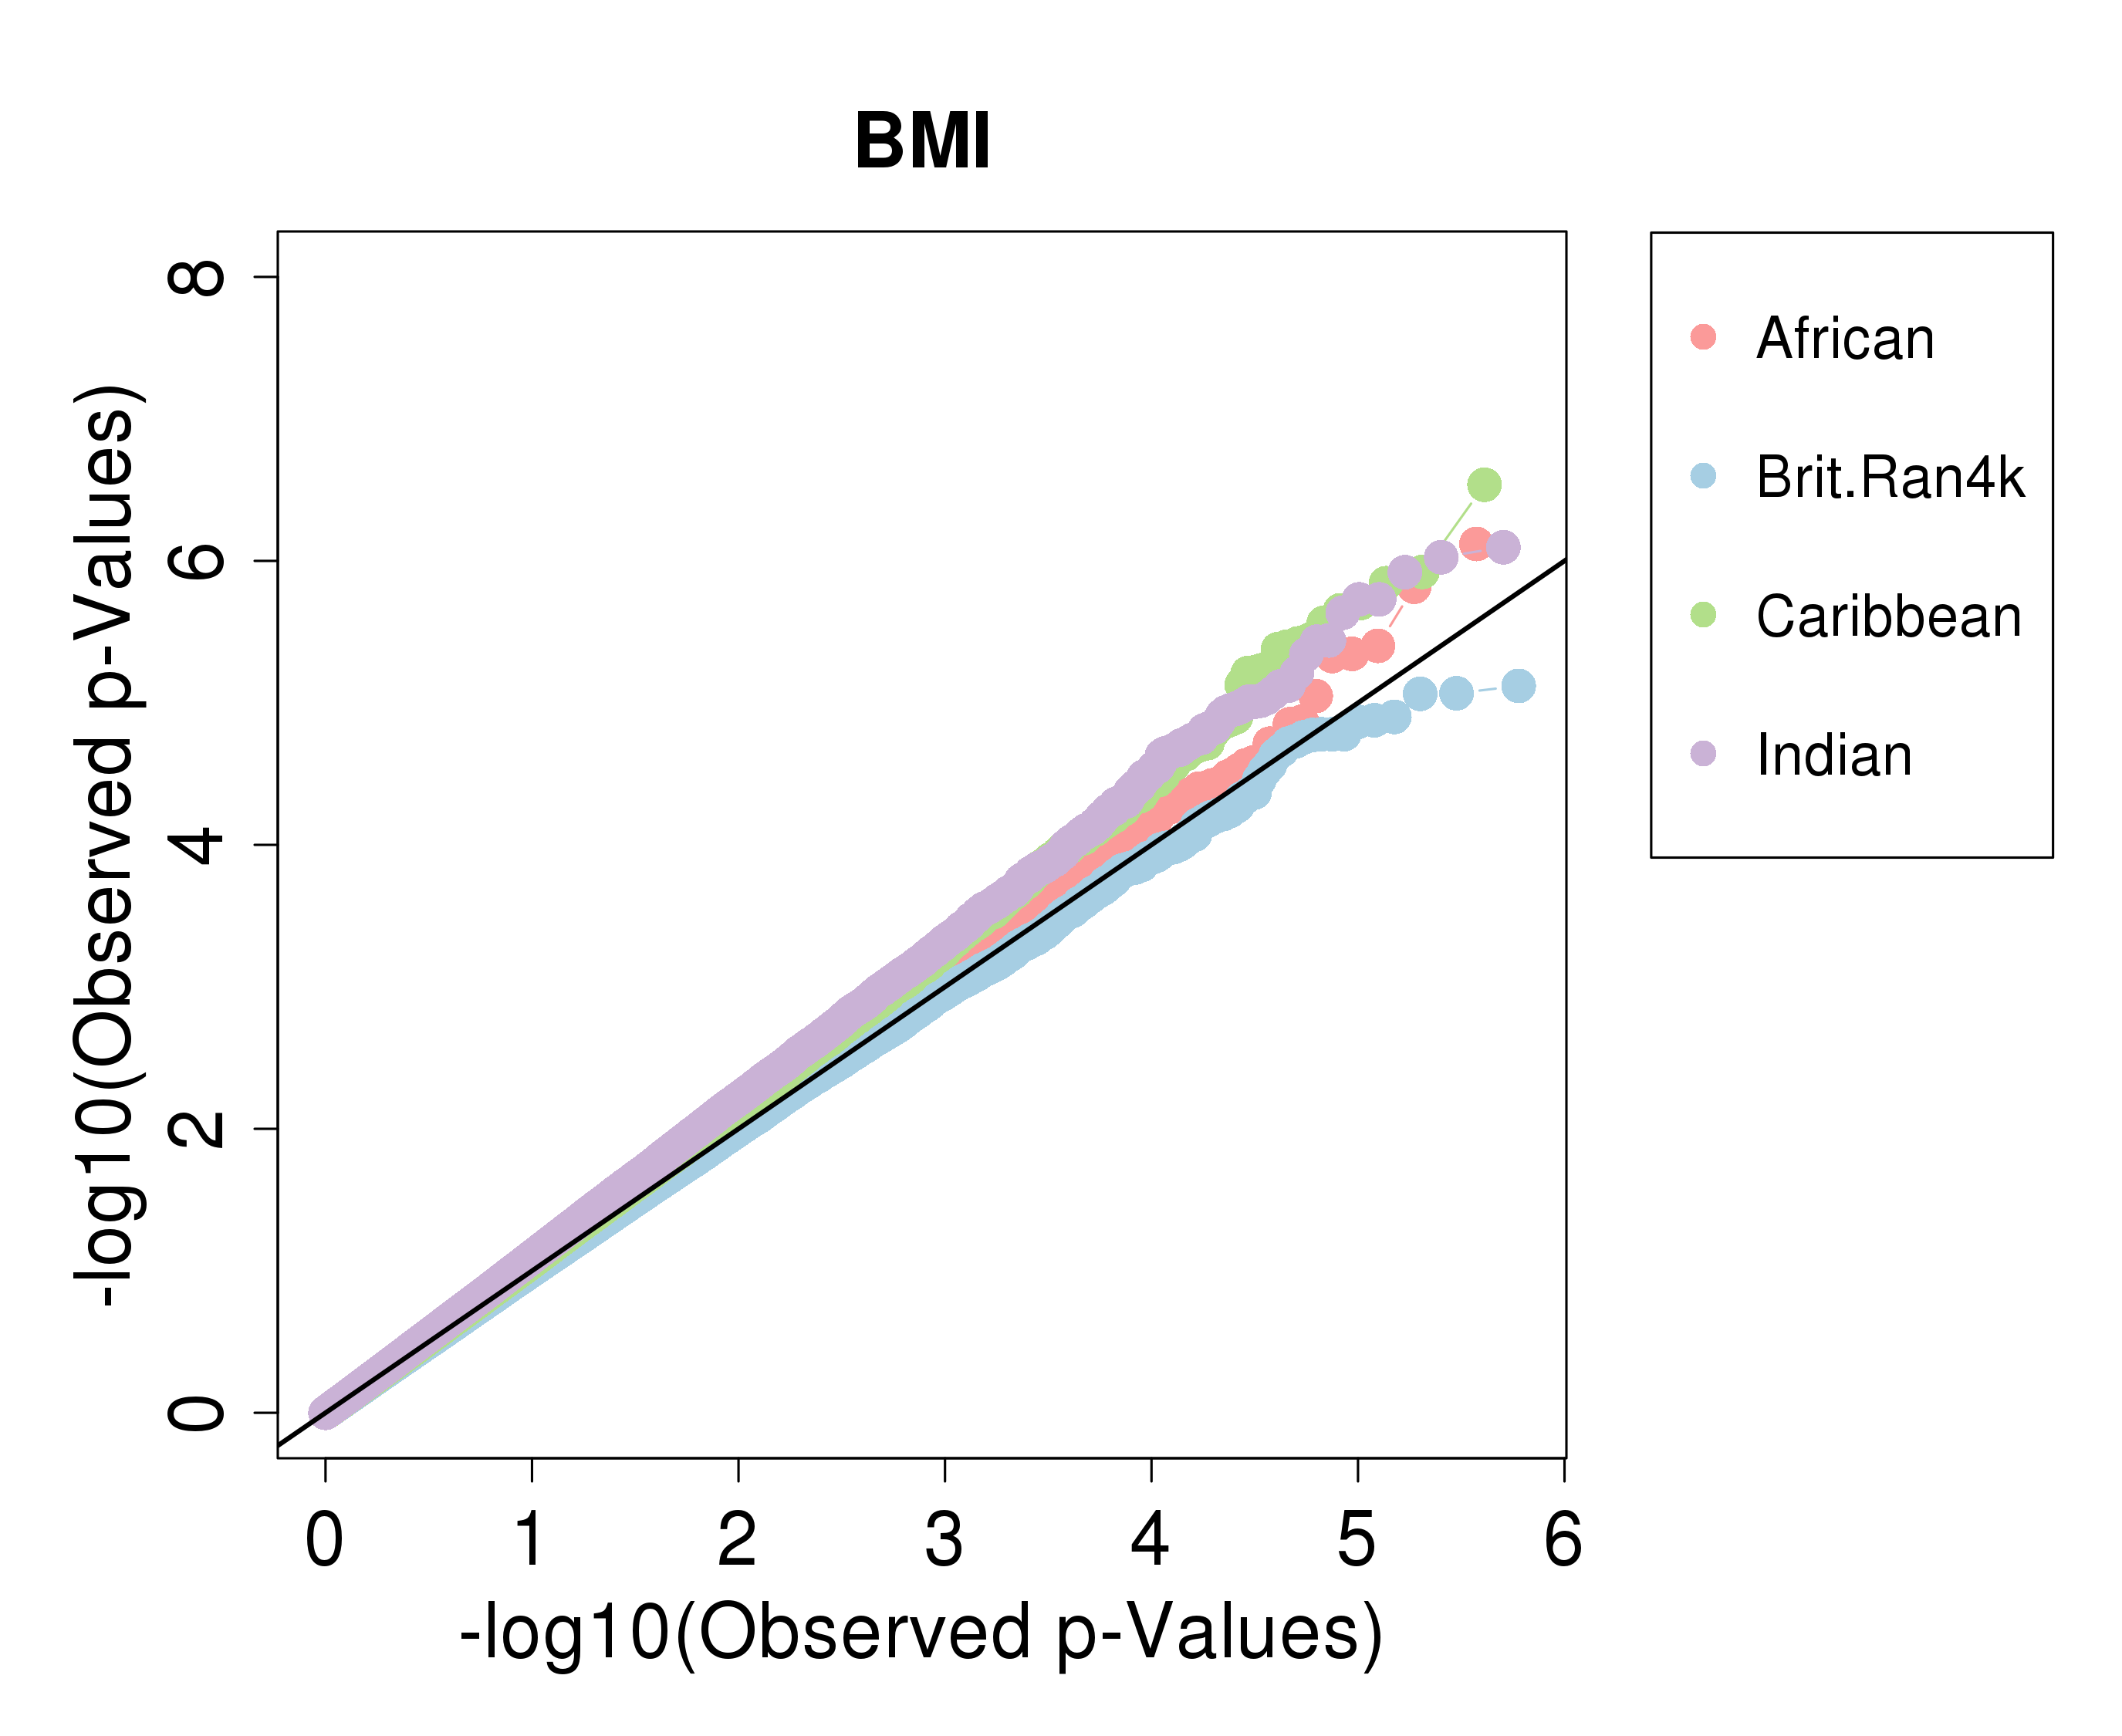
\includegraphics[scale=.5]{Images/Supp/InterPath_Supp_Figure_MAPIT_vs3_BMI.png}
%\caption[TBD]{\textbf{MAPIT Results: BMI QQ-Plots}. The figure shows QQ-plots of our results from running MAPIT on our four initial UKB population subgroups in BMI. On the $x$-axis are the -$\log_{10}$ of the expected $p$-values and the on the $y$-axis are on the -$\log_{10}$ of the observed $p$-values. Each data point is a SNP and total SNP counts per UKB subgroup can be found in Supplementary Table \ref{InterPath-Supp-Table-UKBPopStats}.}
%\label{InterPath-Supp-Figure-MAPIT-BMI}
%\end{figure}
%\clearpage

%\begin{figure}[htbp]
%\centering
%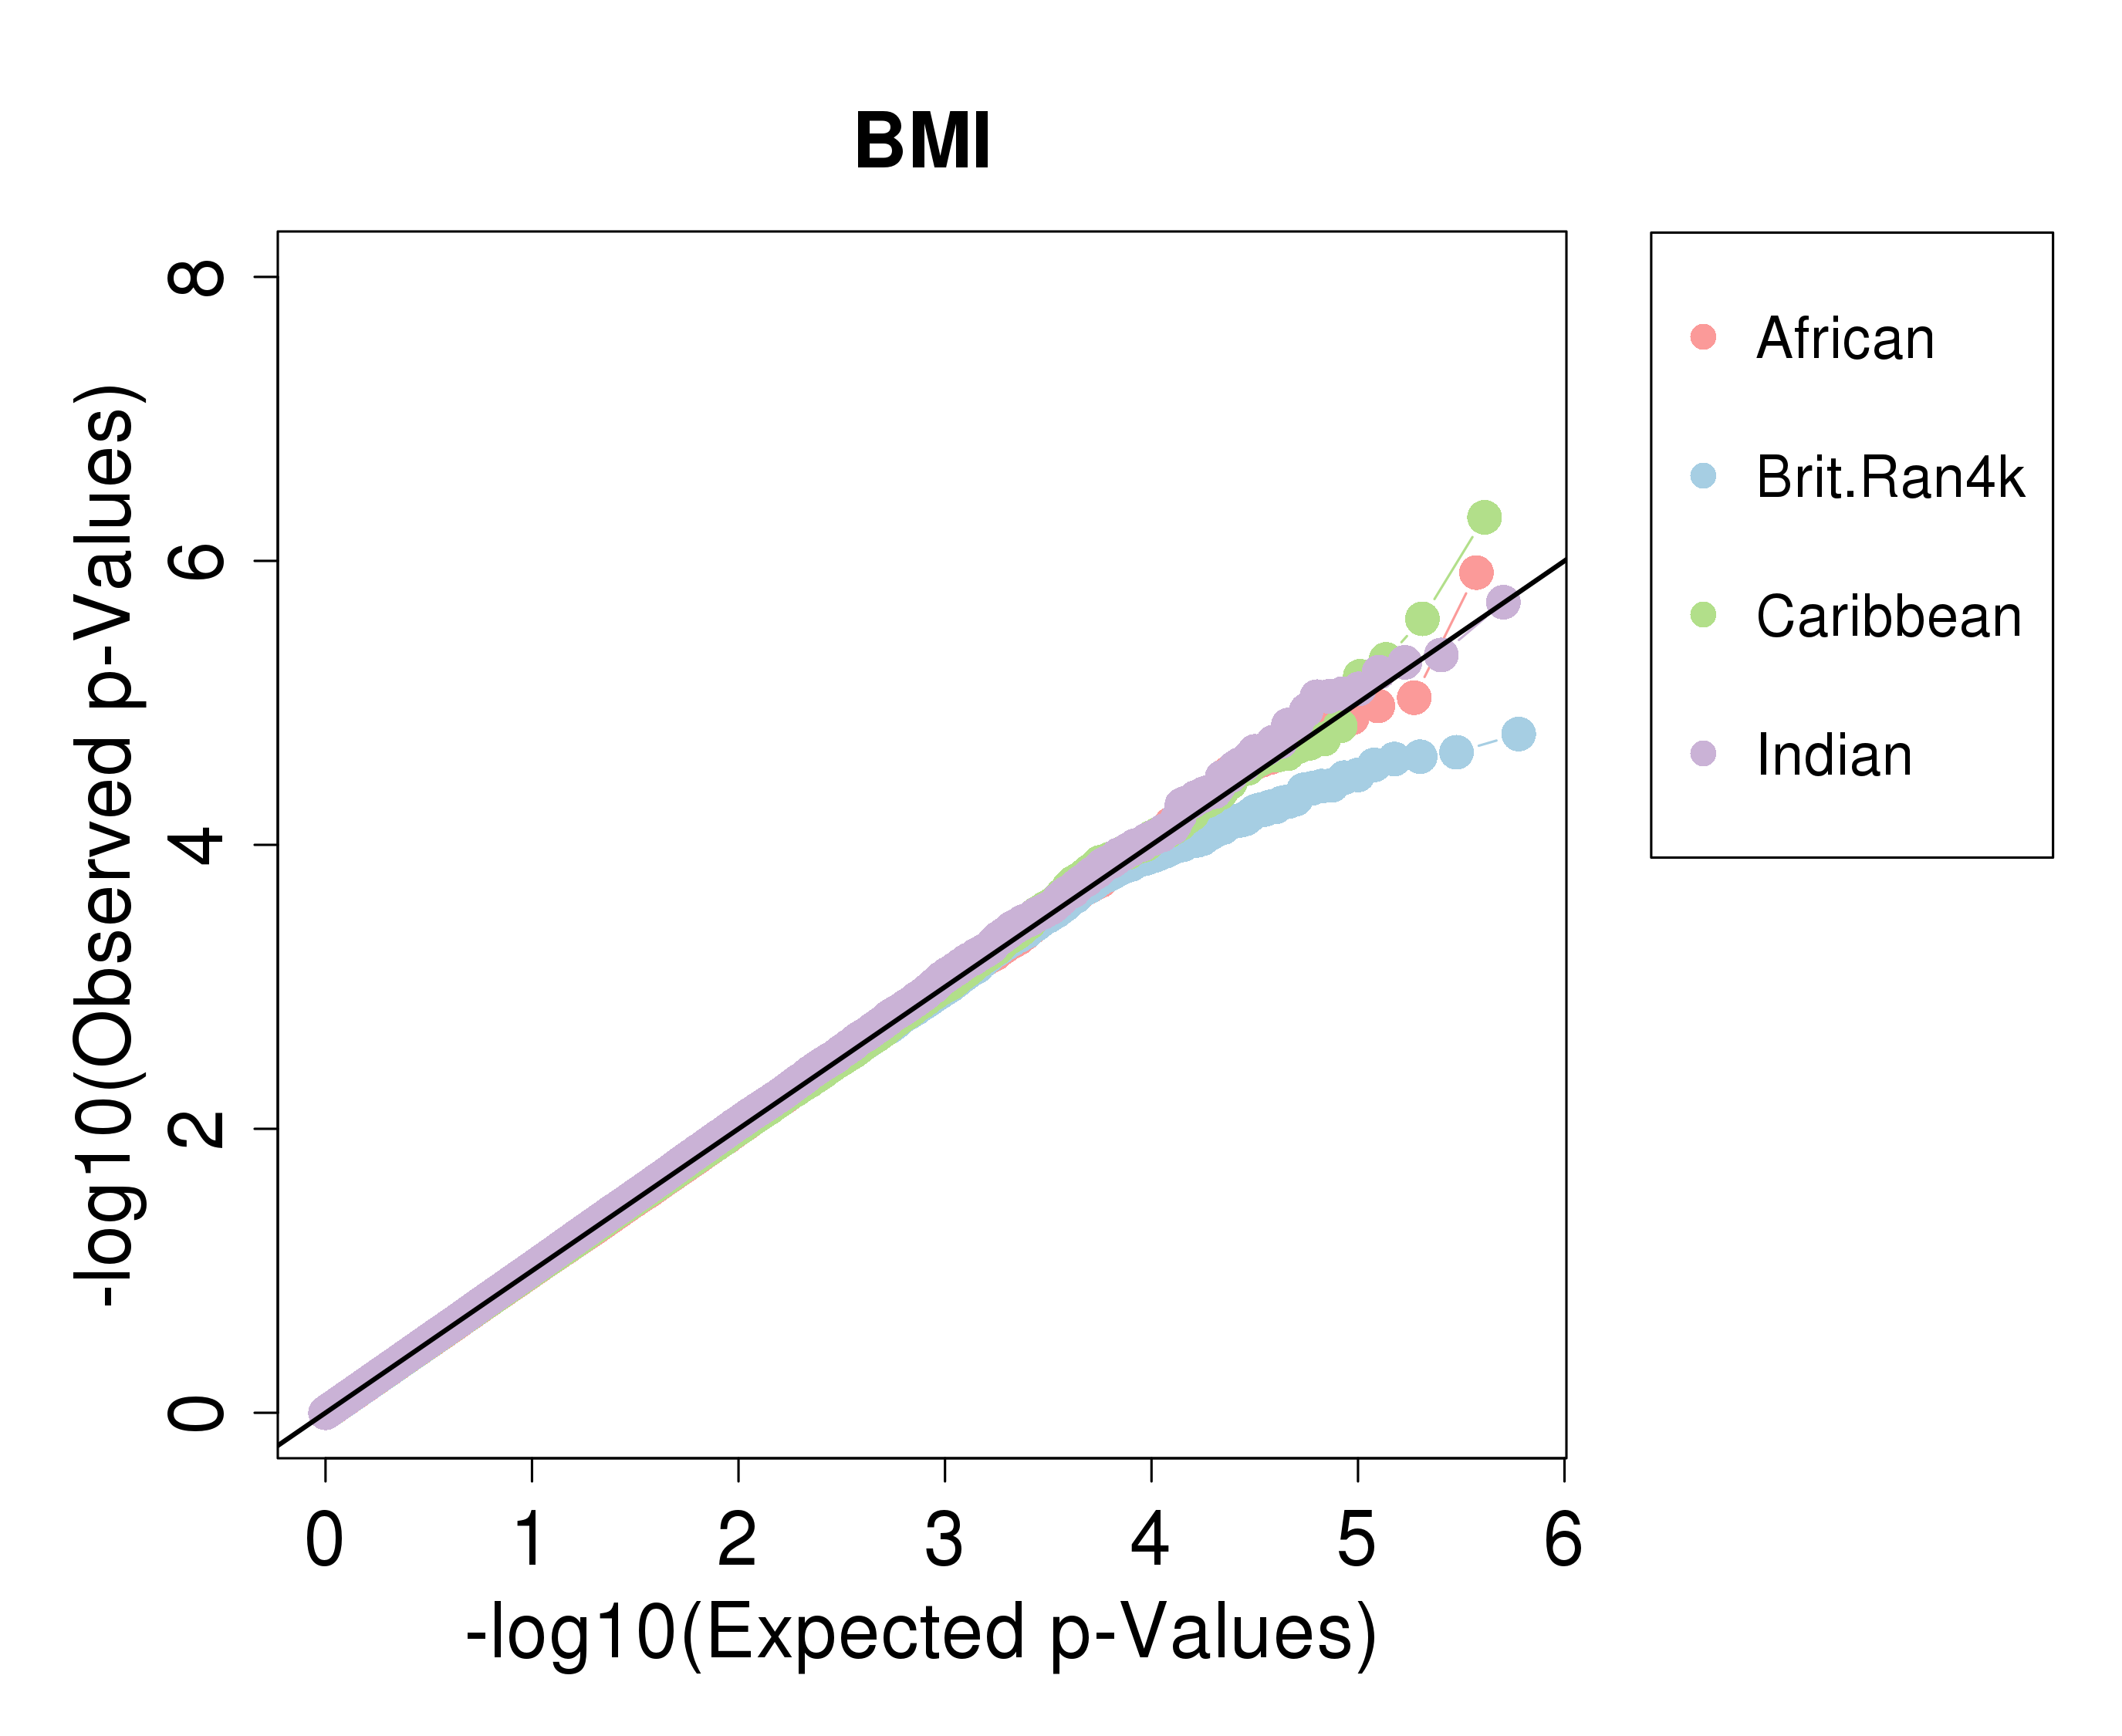
\includegraphics[scale=.35]{Images/Supp/InterPath_Supp_Figure_GWAS_vs2_BMI.png}
%\caption[TBD]{\textbf{GWAS Results QQ-Plots}.}
%\label{InterPath-Supp-Figure-GWAS-BMI}
%\end{figure}
%\clearpage
%
%\begin{figure}[htbp]
%\centering
%\hspace*{-.75cm}
%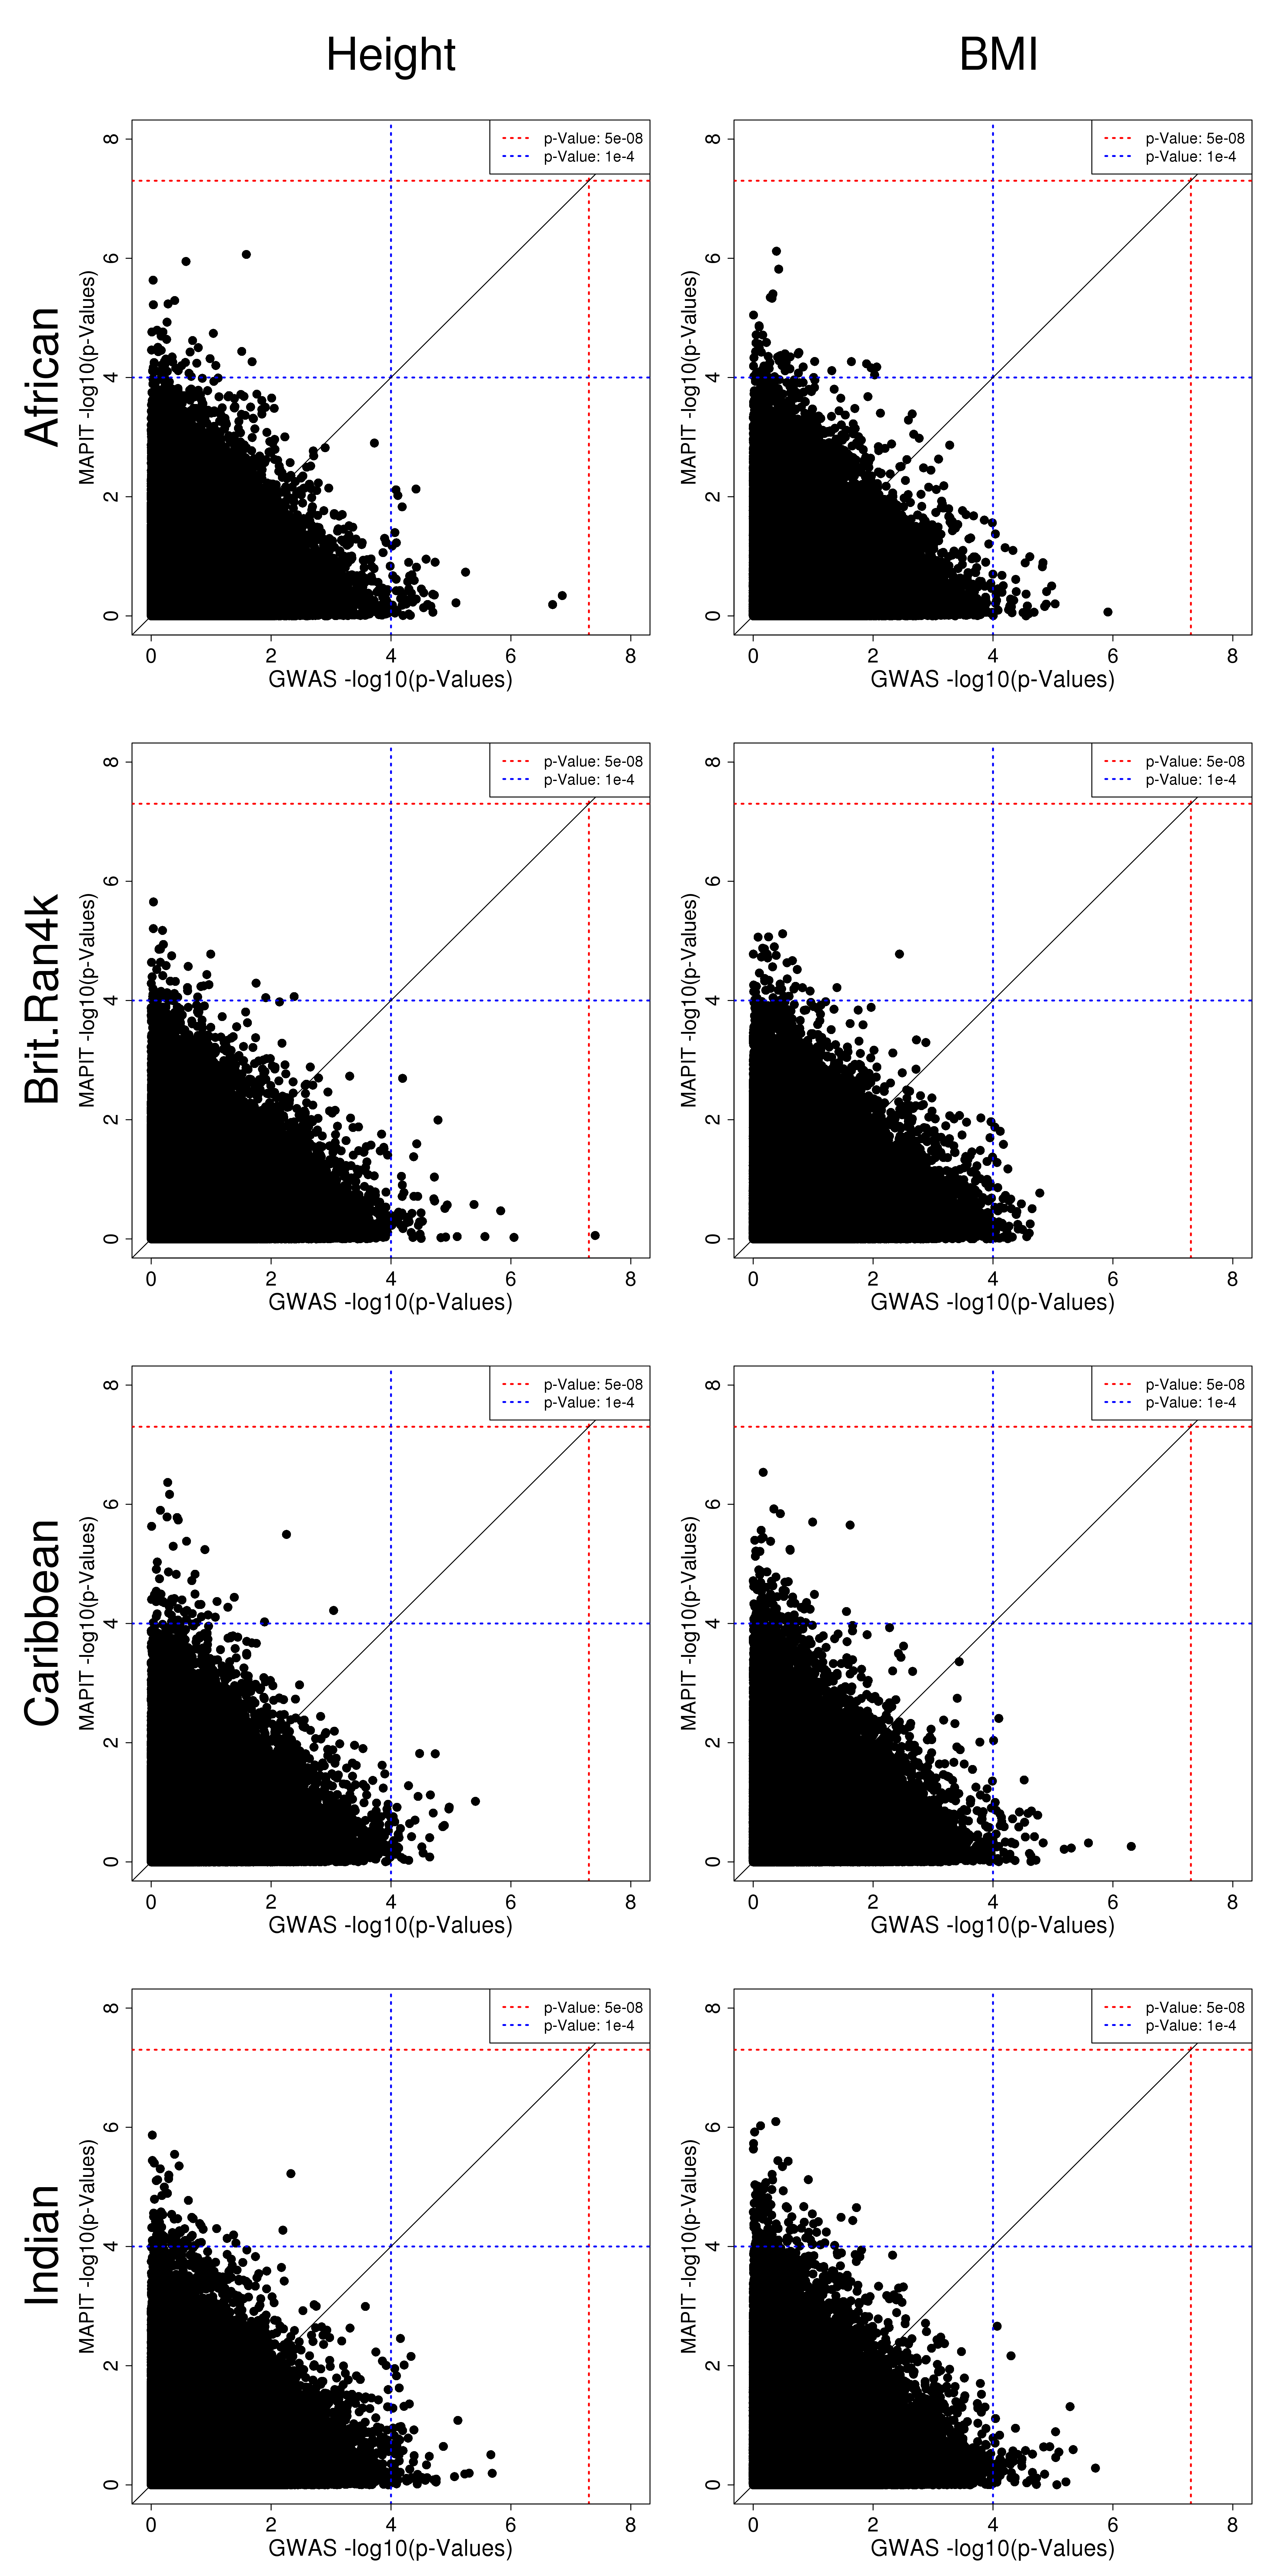
\includegraphics[scale=.3]{Images/Supp/InterPath_Supp_Figure_MAPITvsGWAS_vs2.png}
%\caption[TBD]{\textbf{MAPIT vs. GWAS Results}.}
%\label{InterPath-Supp-Figure-MAPITvsGWAS}
%\end{figure}
%\clearpage

%\setlength{\footskip}{3cm}
%\begin{figure}[htbp]
%\centering
%\vspace*{-2cm}
%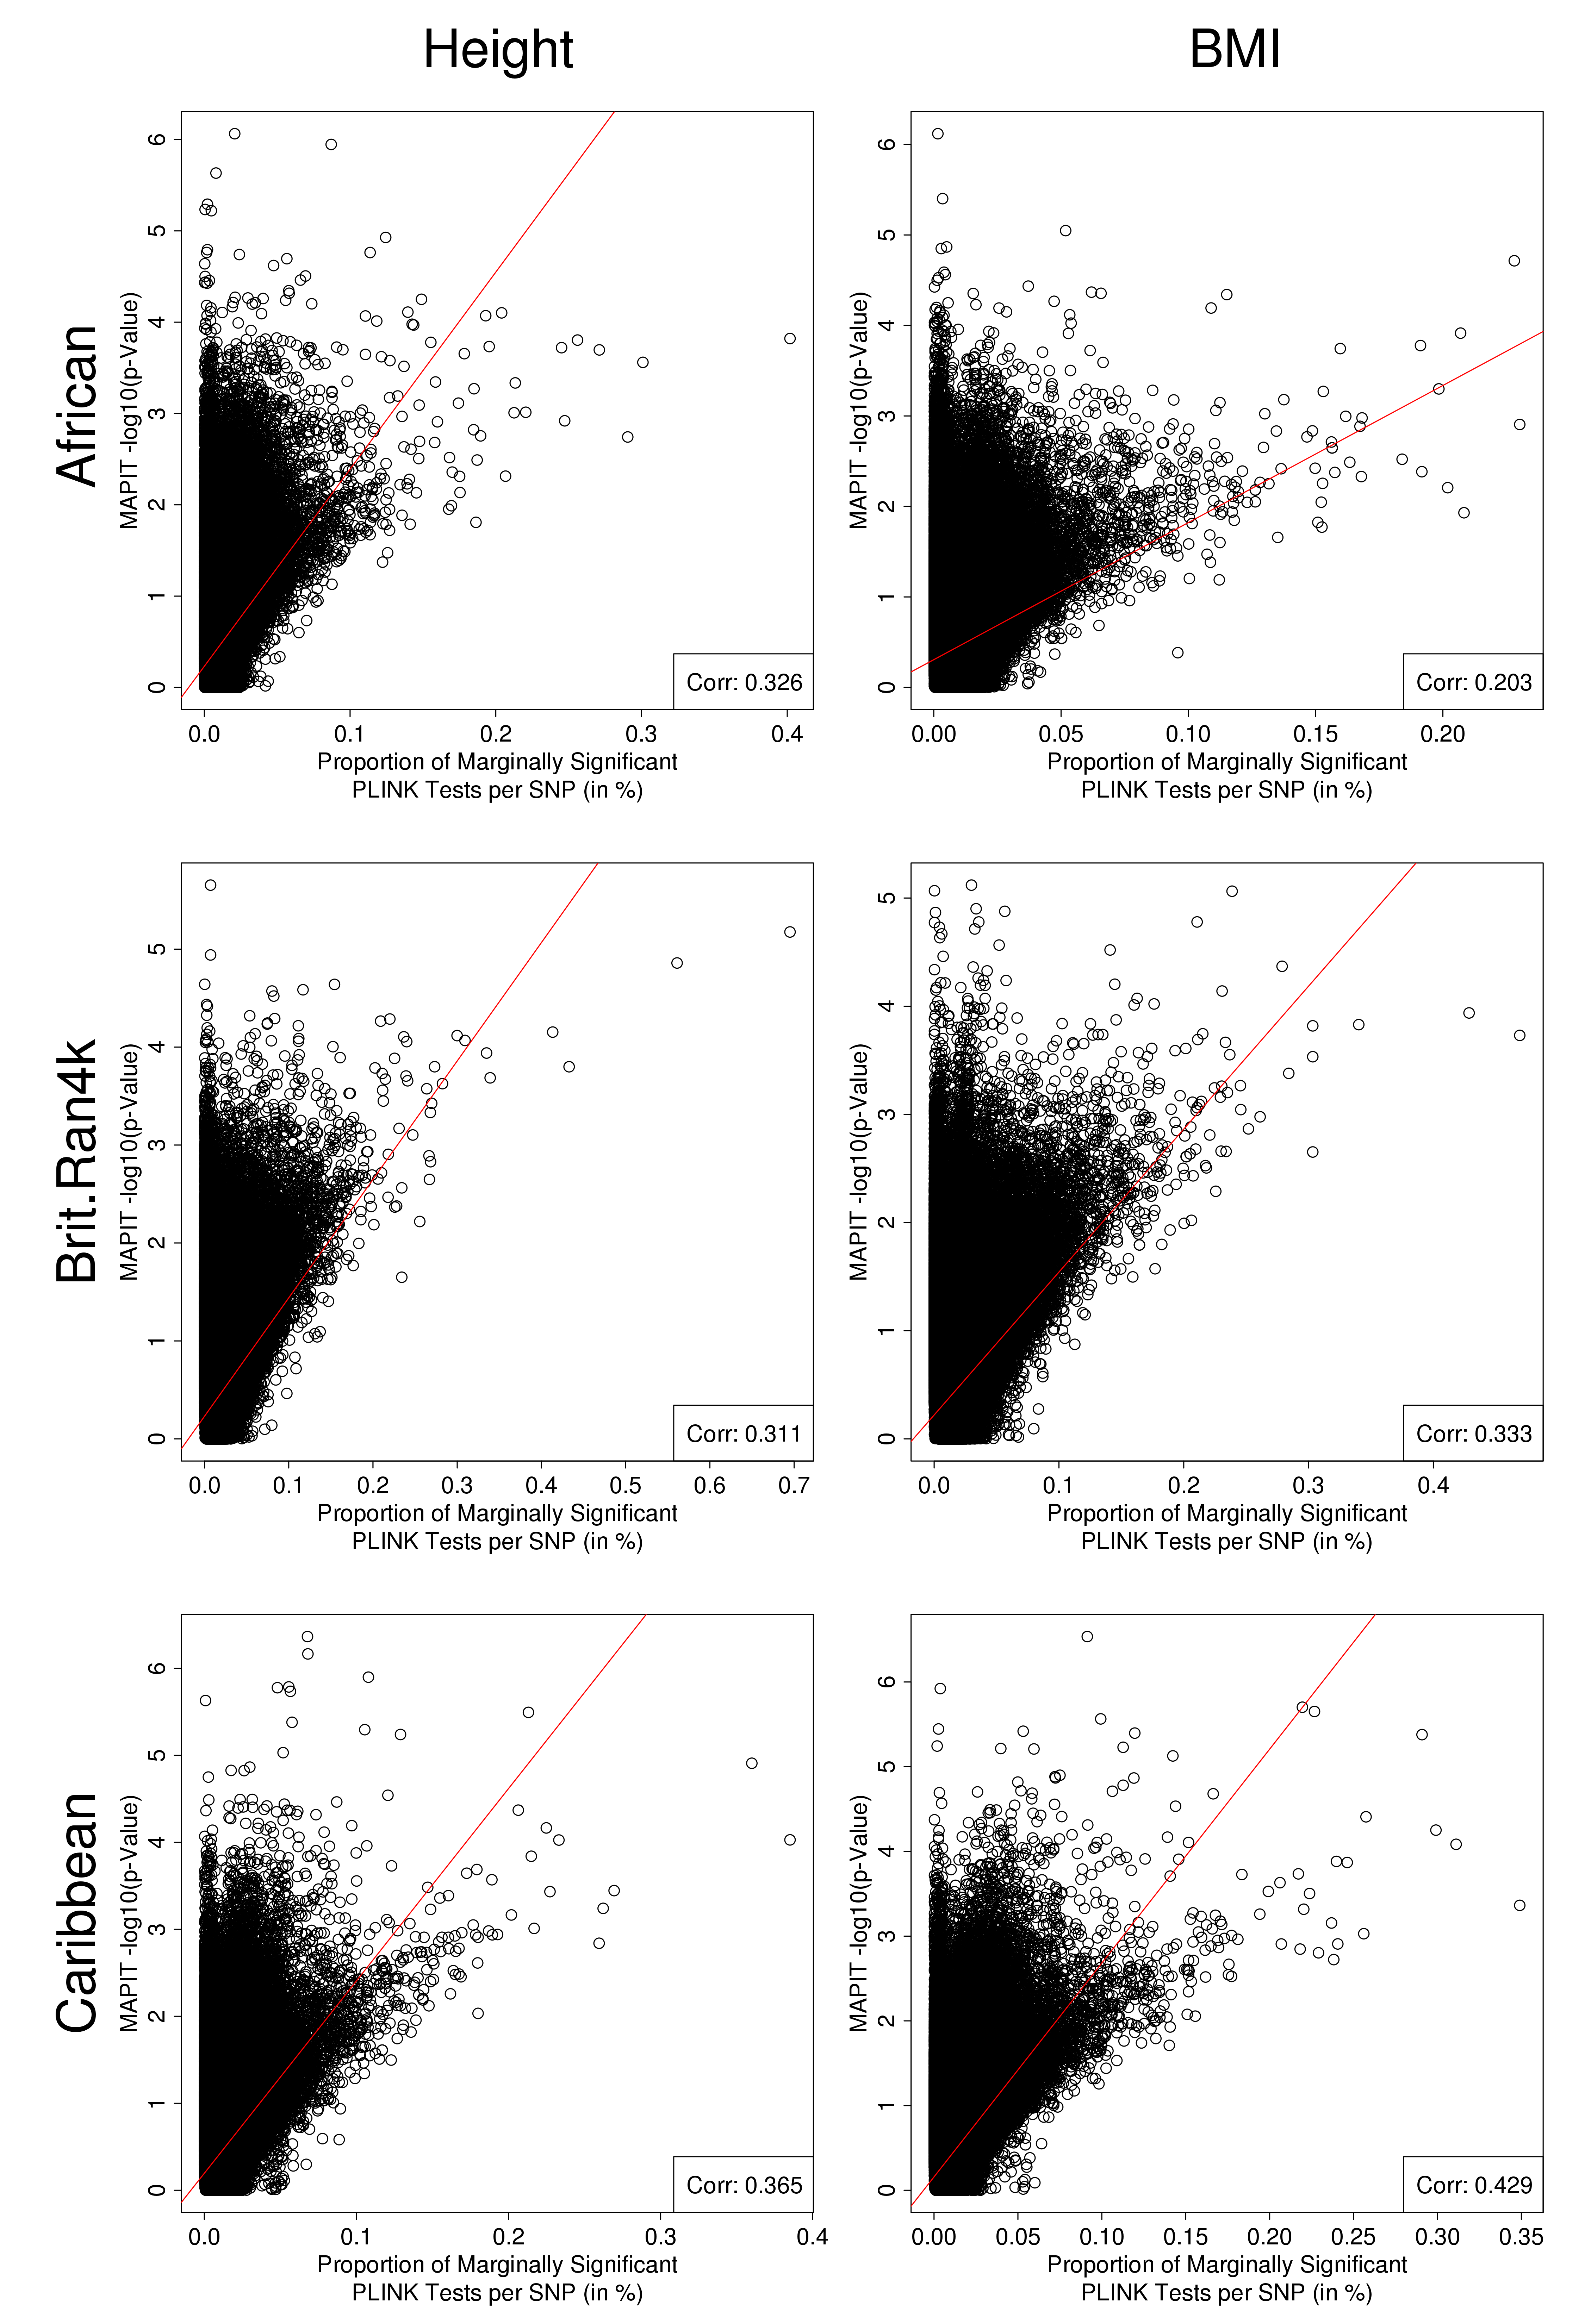
\includegraphics[scale=.3]{Images/Supp/InterPath_Supp_Figure_PLINKvsMAPIT_vs3_AllPops_HeightBMI_pt1.png}
%\caption[TBD]{\textbf{Comparison of single-SNP epistasis methods in height and BMI, per subgroup}. Caption continued at end of figures.}
%\label{InterPath-Supp-Figure-MAPITvsPLINK-HeightBMI-AllPops-a}
%\end{figure}
%\clearpage
%\setlength{\footskip}{1cm}
%\addtocounter{figure}{-1}

%\setlength{\footskip}{3cm}
%\begin{figure}[htbp]
%\centering
%\vspace*{-2cm}
%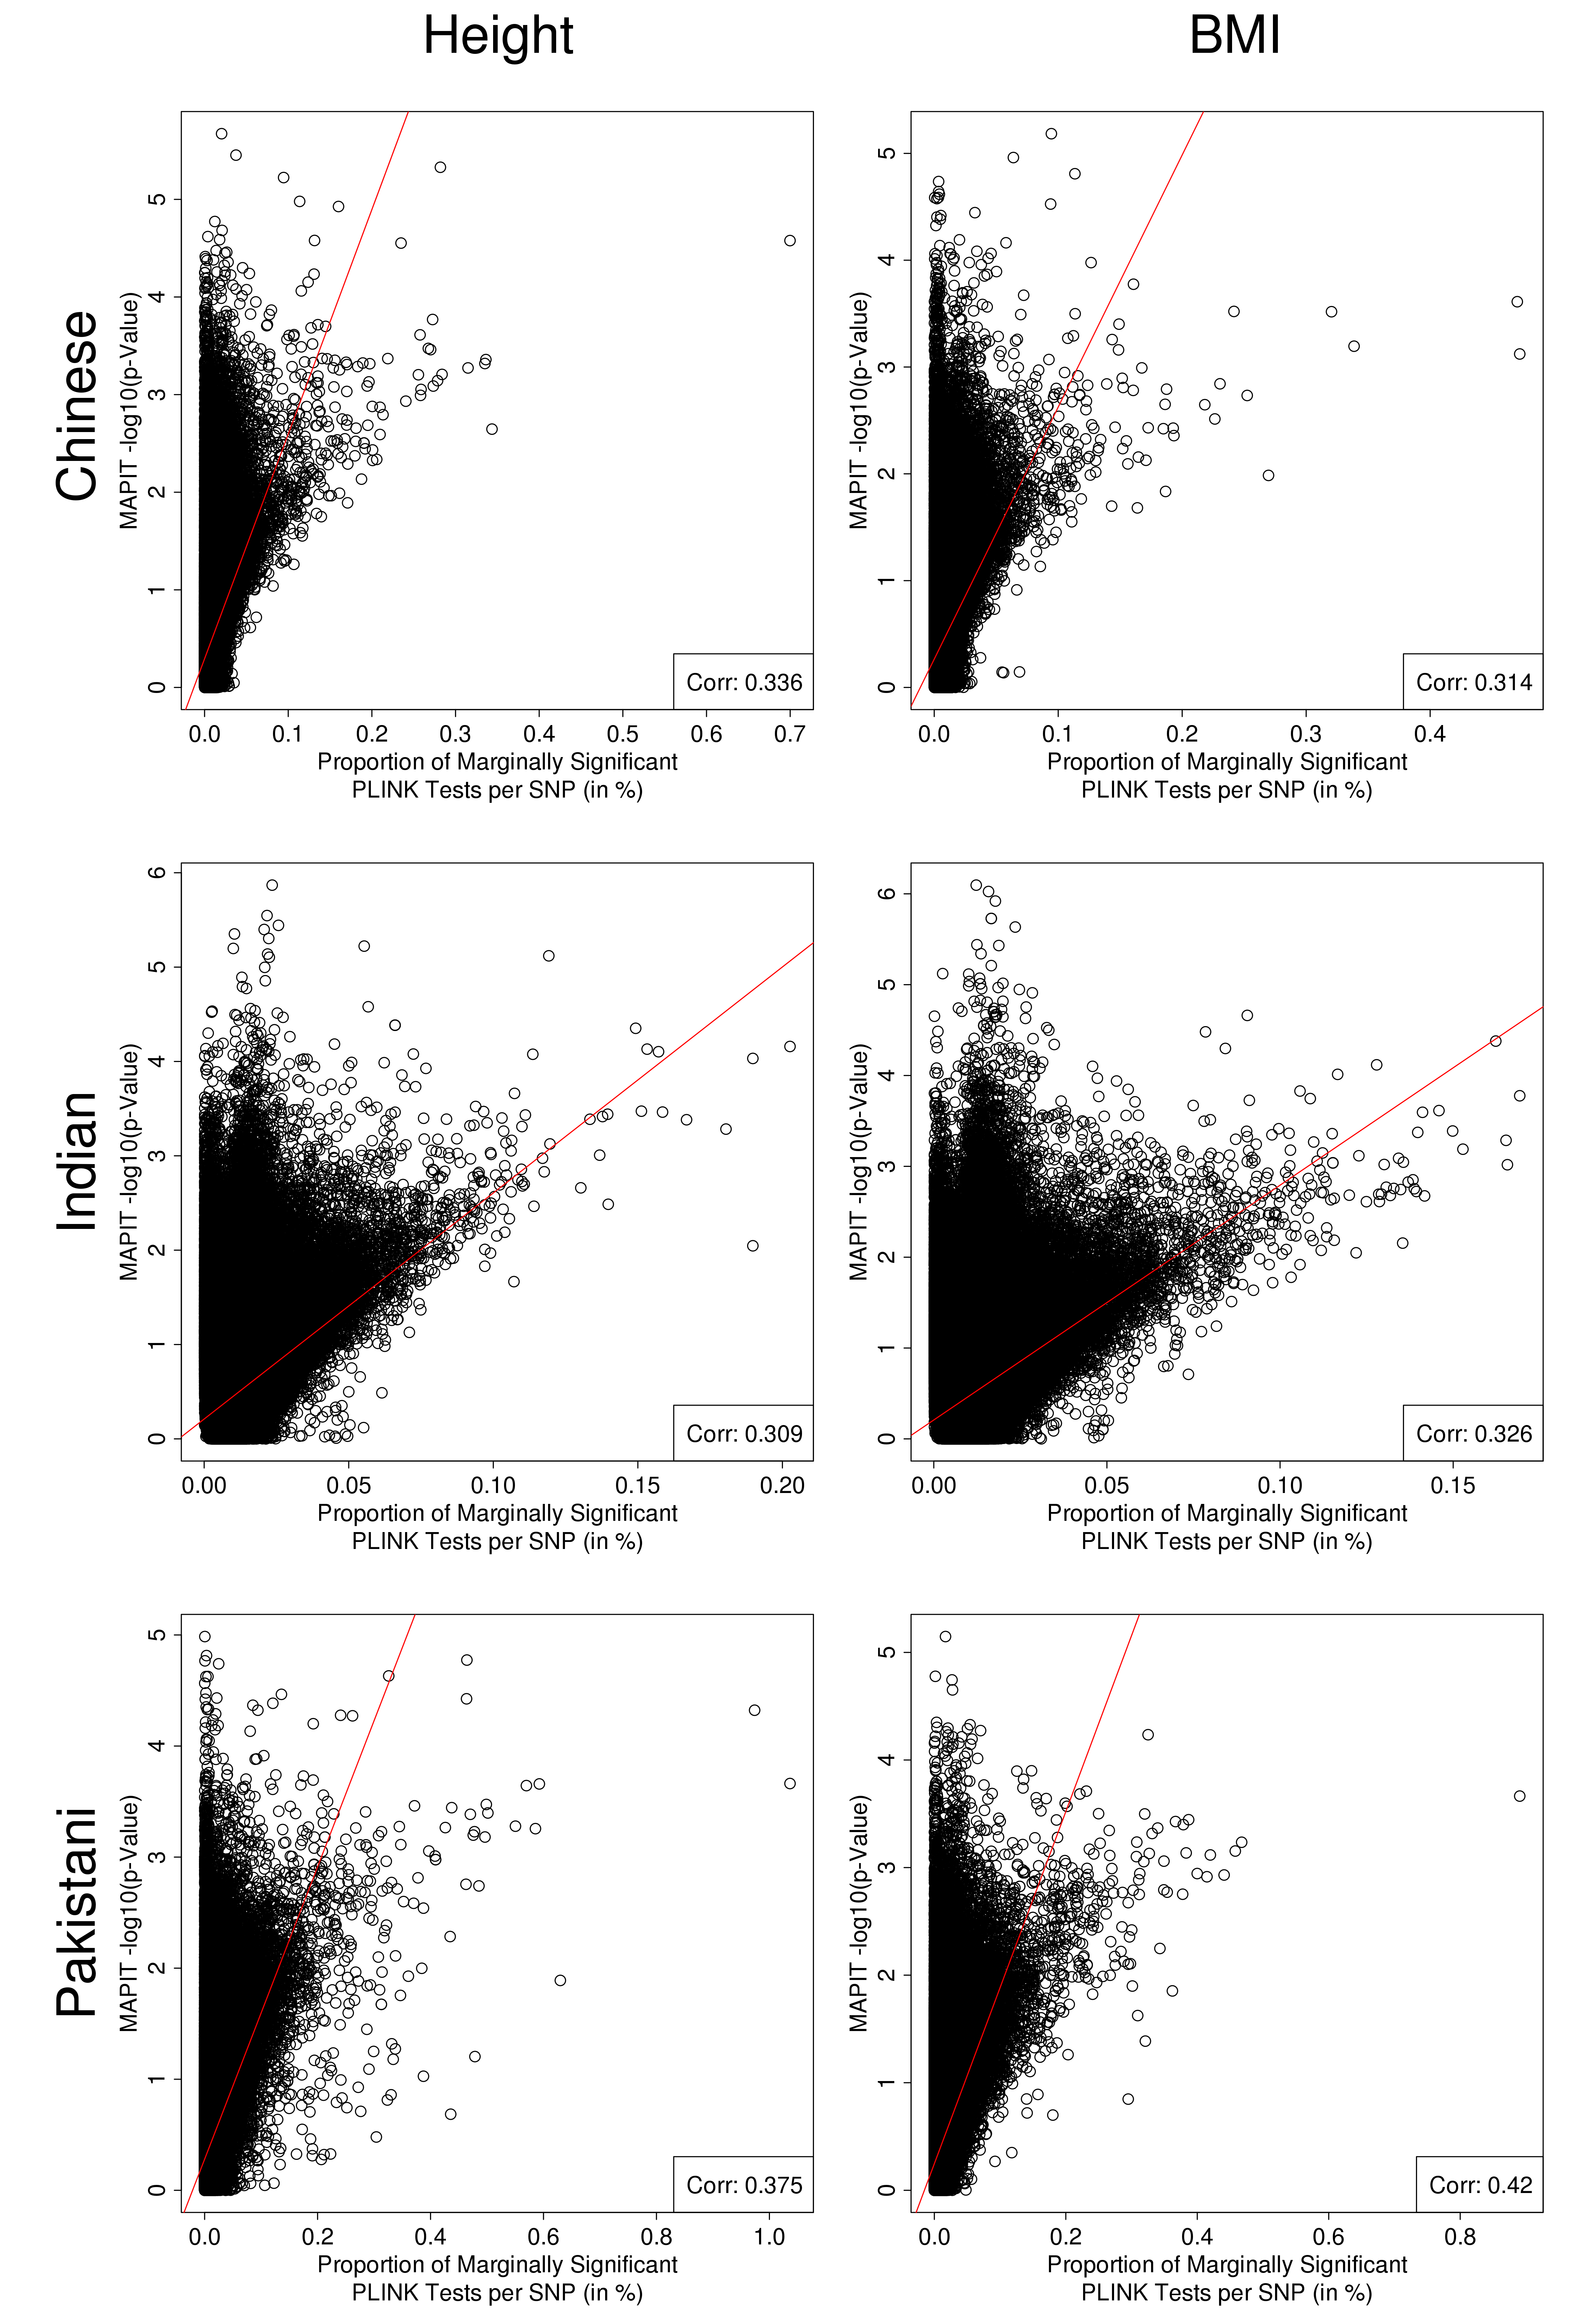
\includegraphics[scale=.3]{Images/Supp/InterPath_Supp_Figure_PLINKvsMAPIT_vs3_AllPops_HeightBMI_pt2.png}
%\caption[TBD]{\textbf{Comparison of single-SNP epistasis methods in height and BMI, per subgroup}. Caption continued at end of figure.}
%\label{InterPath-Supp-Figure-MAPITvsPLINK-HeightBMI-AllPops-b}
%\end{figure}
%\clearpage
%\setlength{\footskip}{1cm}
%\addtocounter{figure}{-1}

%\begin{figure} [t!]
%\caption[TBD]{\textbf{Comparison of single-SNP epistasis methods in height and BMI, per subgroup}. The figure shows the single-SNP PLINK results vs. MAPIT results for height and BMI in each UKB subgroup. For each individual plot, the PLINK results are shown on the $x$-axis as the proportion of marginally significant interactions per SNP (where marginally significant is defined as $p$-value $< 1\times10^{-4}$) and the MAPIT results are shown on the $y$-axis as the -$\log_{10}$ of the MAPIT $p$-values. The dotted red line shows the line of best fit, and the correlation between the two metrics is shown in the legend. For many of these plots we observe a subset of SNPs with greater marginal epistasis (higher -$\log_{10}$ $p$-values) beginning to correlate with having larger proportions of marginally significant SNP-by-SNP interactions. Seeing the same signal between two different approaches suggests there may be evidence for epistasis on the single-SNP level, albeit weak.}
%\label{InterPath-Supp-Figure-MAPITvsPLINK-HeightBMI-All-caption}
%\end{figure}
%\clearpage

%\begin{figure}[htbp]
%\centering
%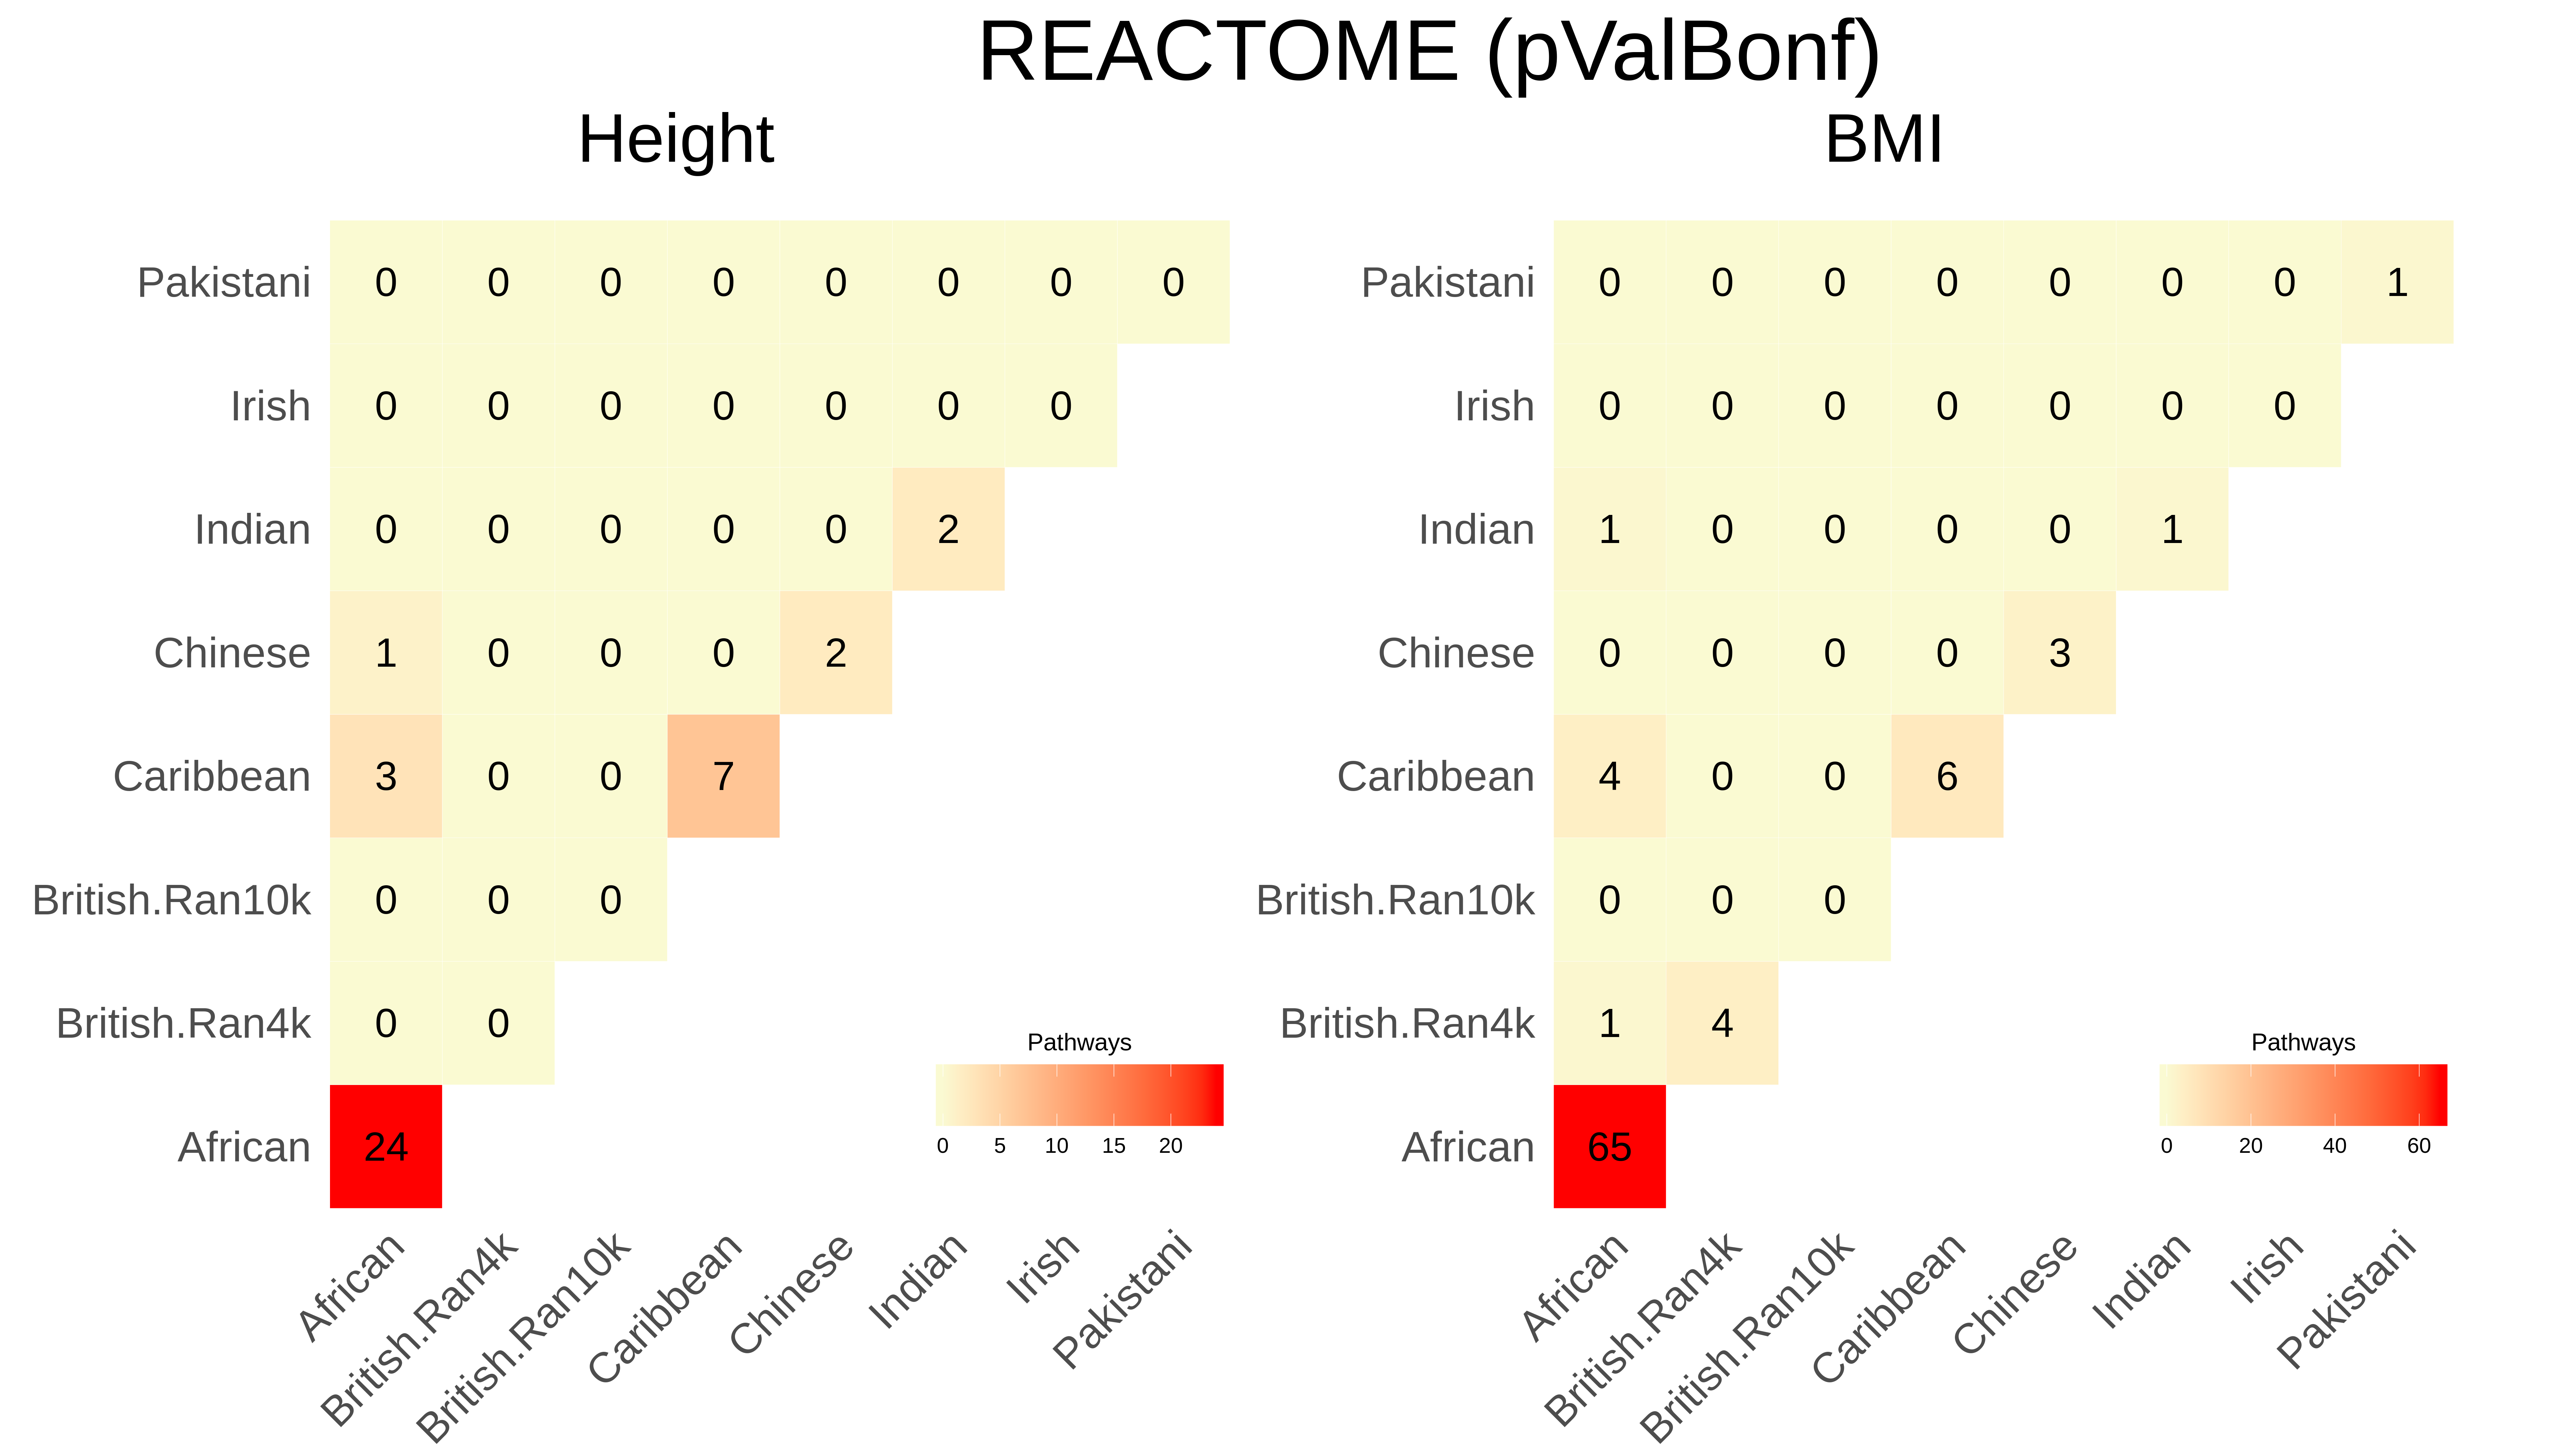
\includegraphics[scale=.225]{Images/Supp/InterPath_Supp_Figure_Heatplots_REACTOME_vs1.png}
%\caption[TBD]{\textbf{TBD}. \\ See above (this would be a supplementary figure).}
%\label{InterPath-Supp-Figure-Heatplots-REACTOME}
%\end{figure}
%\clearpage


%\begin{figure}[htbp]
%\centering
%\includegraphics[scale=.15]{Images/Main/InterPath_Main_PopCompDotPlots_African_vs1.png}
%\caption[]{\textbf{MAPIT-R Cross-Population KEGG $p$-value Comparisons: African}. Shown are comparisons of each population subgroup's MAPIT-R $p$-value for Height and BMI in KEGG against the African subgroup's MAPIT-R $p$-values. On the $x$-axis are the African subgroup's observed -$\log_{10}$ $p$-value and on the $y$-axis is the other population's observed -$\log_{10}$ $p$-value. Dotted red lines represent Bonferroni-corrected $p$-value thresholds for each population/phenotype combination.}
%\label{InterPath-Main-Figure-PopCompDotPlots}
%\end{figure}
%\clearpage

%\begin{figure}[htbp]
%\centering
%\includegraphics[scale=.15]{Images/Supp/InterPath_Supp_Figure_PhenoCompDotPlots_vs1.png}
%\caption[TBD]{\textbf{MAPIT-R Phenotype $p$-value Comparisons}. \\ Shown is a comparison of the MAPIT-R $p$-values for both phenotypes analyzed across all population subgroups in the KEGG database. Shown on the $x$-axis is the observed height -$\log_{10}$ MAPIT-R $p$-value and shown on the $y$-axis is the observed BMI -$\log_{10}$ MAPIT-R $p$-value. Dotted red lines represent Bonferroni-corrected $p$-value thresholds for each population/phenotype combination (.05 / number of KEGG pathways analyzed). In general we observe a correlation between MAPIT-R $p$-values between each phenotype. In the African subgroup, where we have the most observed power, we find pathways that are significant in both phenotypes as well as each phenotype separately. Additionally, we observe, among marginally significant pathways, stronger MAPIT-R signals in BMI than height -- this is in line with previous observations that BMI may contain higher levels of epistasis than height (citations).}
%\label{InterPath-Supp-Figure-PhenoCompDotPlots}
%\end{figure}
%\clearpage


%\begin{figure}[htbp]
%\centering
%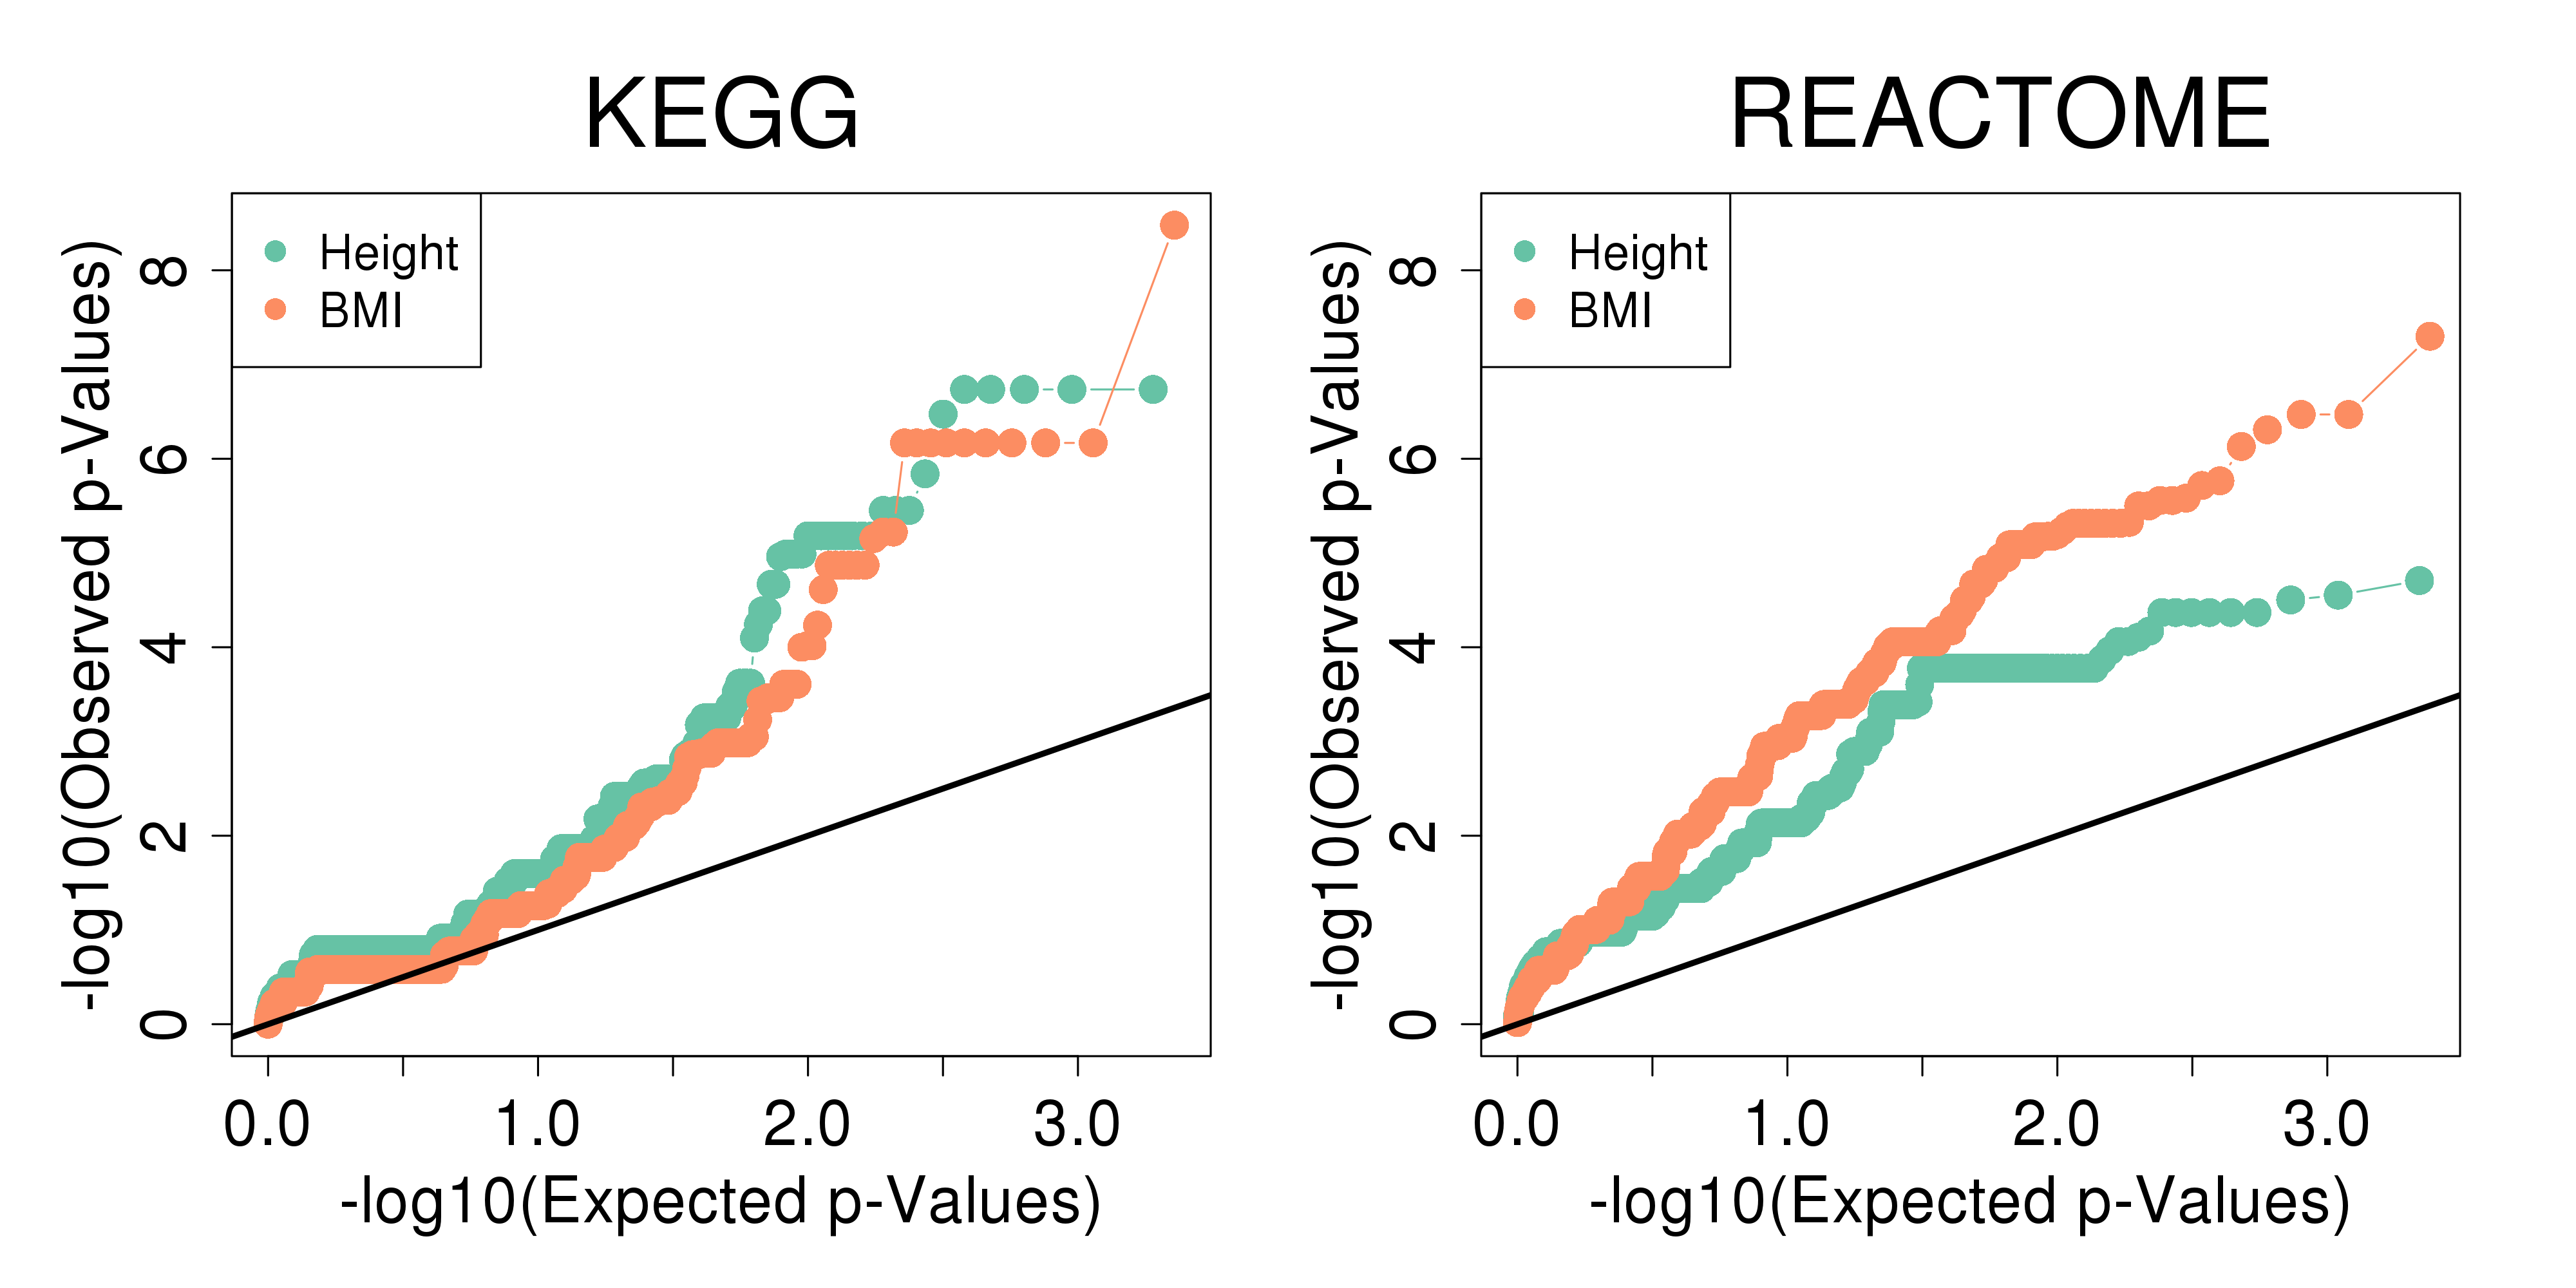
\includegraphics[scale=.45]{Images/Supp/InterPath_Supp_Figure_Hypergeometric_QQPlots_African_vs2.png}
%\caption[TBD]{\textbf{QQ-Plots of gene-based hypergeometric enrichment test $p$-values in the African subgroup}. The figure shows QQ-plots of the gene-based hypergeometric enrichment results for the African subgroup in both height and BMI in both the KEGG (left) and REACTOME (right) databases. Every gene present in the set of MAPIT-R genome-wide significant pathways for that phenotype and pathway database combination was tested, including genes that were only present once. The $x$-axis is the expected -$\log_{10}$ $p$-values and the $y$-axis is the observed -$\log_{10}$ $p$-values.}
%\label{InterPath-Supp-Figure-Hypergeometric-QQPlots-African}
%\end{figure}
%\clearpage

%\begin{figure}[htbp]
%\centering
%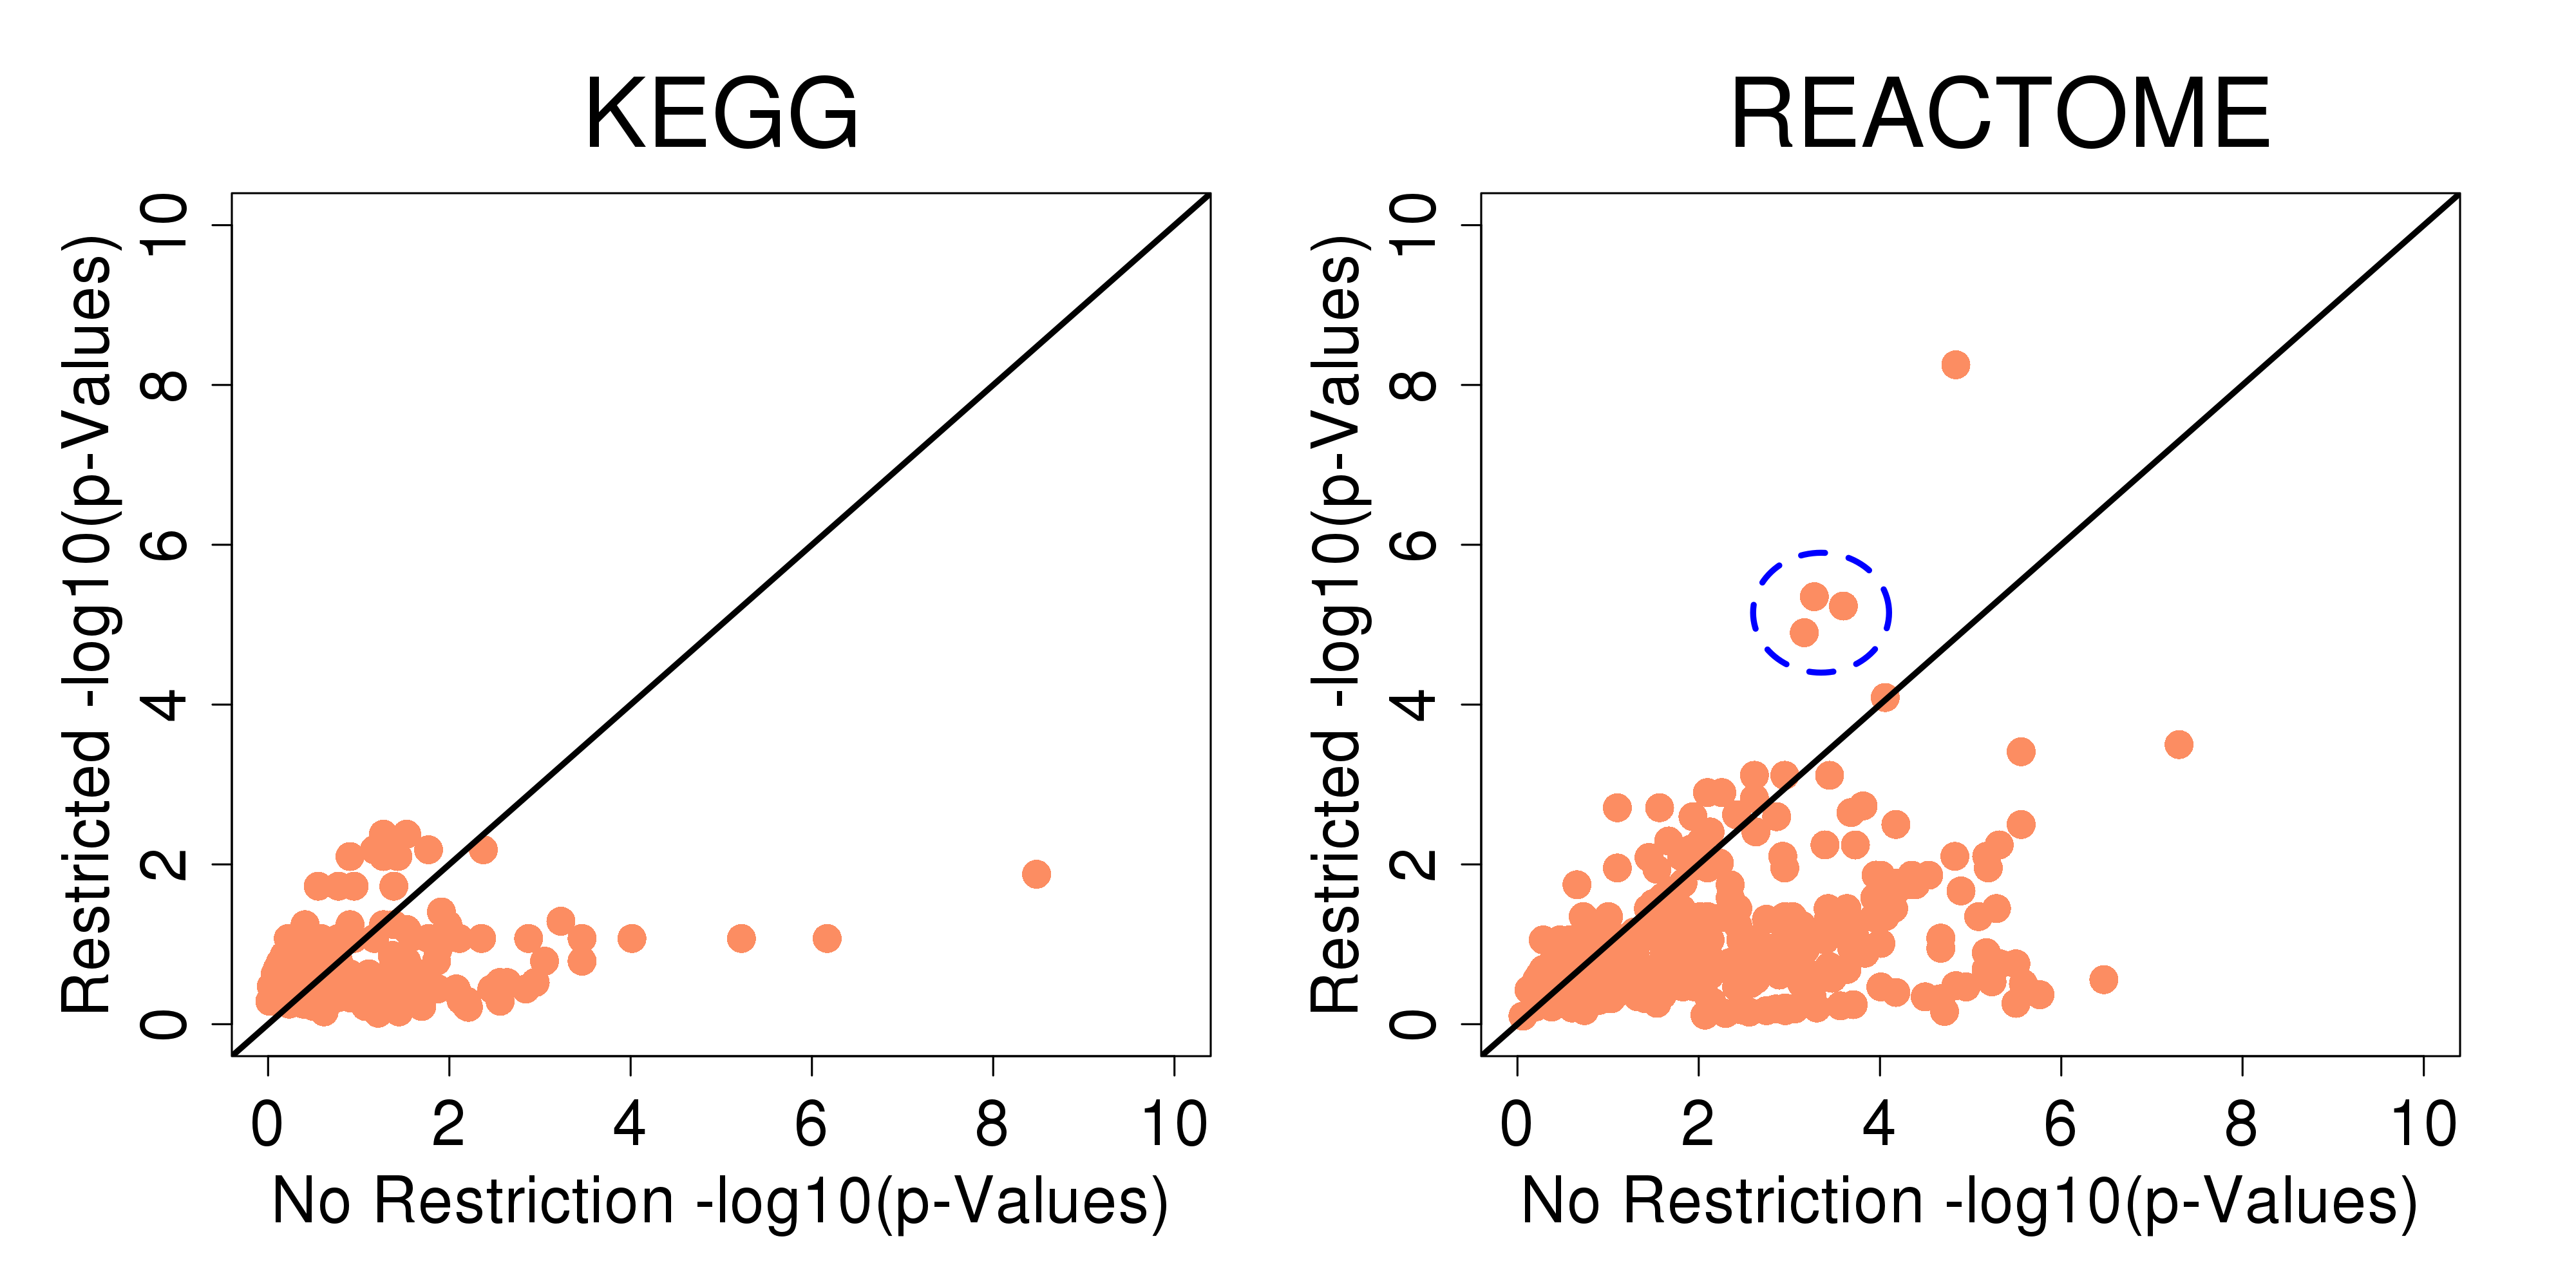
\includegraphics[scale=.45]{Images/Supp/InterPath_Supp_Figure_Hypergeometric_RestrictedComps_African_BMI_vs2.png}
%\caption[TBD]{\textbf{Comparison of gene count hypergeometric enrichment $p$-values in BMI using pathway size restrictions versus no size restrictions in the African subgroup}. The figure shows comparisons of the gene count hypergeometric enrichment $p$-values between the size restricted version of the analysis and the original unrestricted version of the analysis. The size restricted version of the analysis is redoing the hypergeometric enrichment tests but only using pathways that contained $<$ 1,000 SNPs. Only results for BMI are shown here since almost all Bonferroni significant pathways were lost in the height results due to this size restriction step. The $x$-axis shows the original, unrestricted hypergeometric -$\log_{10}$ $p$-values, and the $y$-axis shows the new, size restricted hypergeoemtric -$\log_{10}$ $p$-values. The PSM* gene cluster is highlighted in the REACTOME plot. For lists of the top genes that became more significant due to the size restriction step, see Supplementary Table \ref{InterPath-Supp-Table-Hypergeometric-RestrictedComps-African-BMI-TopExamples}.}
%\label{InterPath-Supp-Figure-Hypergeometric-RestrictedComps-African-BMI}
%\end{figure}
%\clearpage



%\begin{landscape}
%\begin{figure}[htbp]
%\centering
%\hspace*{-2.5cm}
%\vspace*{-1cm}
%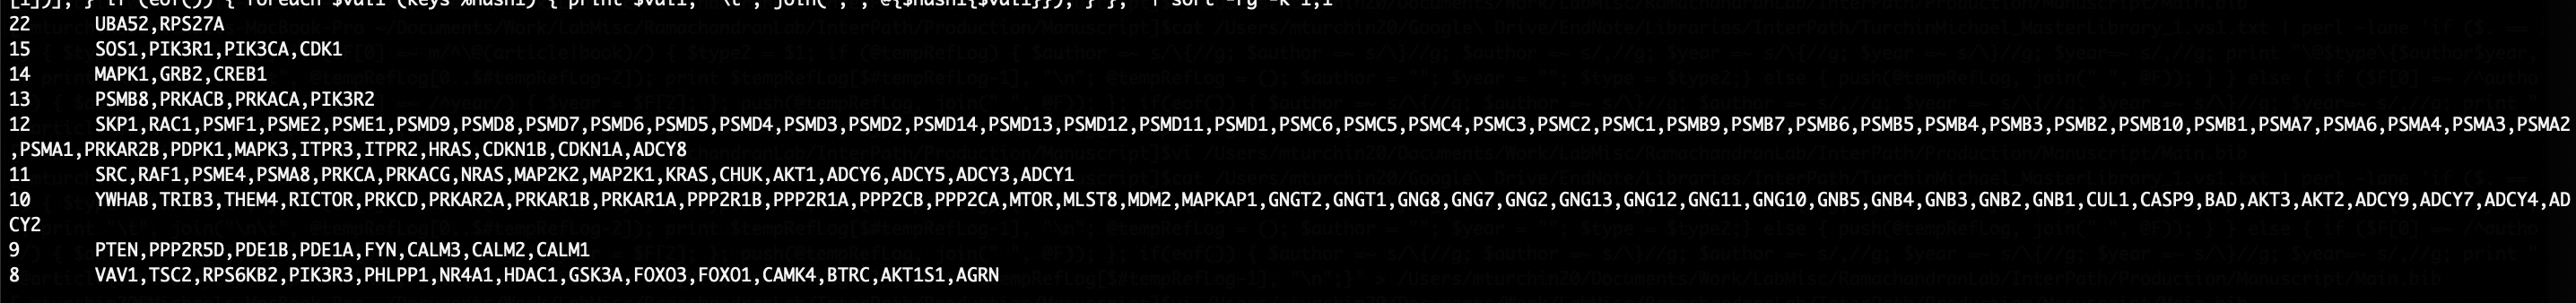
\includegraphics[scale=1]{Images/Supp/InterPath_Supp_Table_TopPathwayGeneCounts.png}
%\caption[TBD]{\textbf{Table of Most Present Genes in Significant MAPIT-R Pathways} \textcolor{red}{this will be a table}}
%\label{InterPath-Supp-Table-GeneCounts}
%\end{figure}
%\end{landscape}
%\clearpage


%\begin{landscape}
%\setlength{\footskip}{2cm}
%\begin{table}[ht]
%\centering
%\begin{tabular}{lrrr}
%  \hline
%\textbf{Pathway} & \textbf{Genes} & \textbf{SNPs} & %\textbf{$p$-Value} \\ 
%  \hline
%REACTOME\_M\_G1\_TRANSITION & 73 & 458 & 3.191E-06 \\ 
%  REACTOME\_CELL\_CYCLE\_CHECKPOINTS & 105 & 670 & 5.781E-06 \\ 
%  REACTOME\_HOST\_INTERACTIONS\_OF\_HIV\_FACTORS & 112 & 963 & 7.521E-06 \\ 
%  REACTOME\_DOWNSTREAM\_SIGNALING\_EVENTS\_OF\_ & & & \\ 
%  \qquad B\_CELL\_RECEPTOR\_BCR & 89 & 745 & 1.195E-05 \\
%  REACTOME\_REGULATION\_OF\_APOPTOSIS & 52 & 564 & 1.218E-05 \\ 
%  REACTOME\_MITOTIC\_G1\_G1\_S\_PHASES & 121 & 747 & 1.453E-05 \\ 
%  REACTOME\_ACTIVATION\_OF\_NF\_KAPPAB\_IN\_B\_CELLS & 59 & 465 & 1.861E-05 \\ 
%  REACTOME\_ASSEMBLY\_OF\_THE\_PRE\_REPLICATIVE\_COMPLEX & 60 & 331 & 3.293E-05 \\ 
%  REACTOME\_ANTIGEN\_PROCESSING\_CROSS\_PRESENTATION & 68 & 850 & 3.956E-05 \\ 
%   \hline
%\end{tabular}
%  \caption{\textbf{Size-restricted pathways that contain the PSM* cluster of genes}. Caption continued on next page.}
%\label{InterPath-Supp-Table-AllPops-TopGeneCount-SizeRestricted-Proteasome}
%\end{table}
%\clearpage
%\end{landscape}
%\setlength{\footskip}{1cm}

%\addtocounter{table}{-1}
%\begin{table} [t!]
%  \caption{\textbf{Size-restricted pathways that contain the PSM* cluster of genes}. The table shows the MAPIT-R genome-wide significant REACTOME pathways for BMI in the African subgroup that both have SNP sizes less than 1,000 and also contain the set of proteasome genes being investigated (\textit{PSMA}*, \textit{PSMB}*, \textit{PSMC}*, \textit{PSMD}*, and \textit{PSME*}). The first column shows the REACTOME pathway names, the second column shows the number of genes that were included in the MAPIT-R analysis, the third column show the number of SNPs that were included in the MAPIT-R analysis, and the fourth column shows the MAPIT-R $p$-value.}
%\label{InterPath-Supp-Table-AllPops-TopGeneCount-SizeRestricted-Proteasome-Caption}
%\end{table}
%\clearpage

%\begin{figure}[htbp]
%\centering
%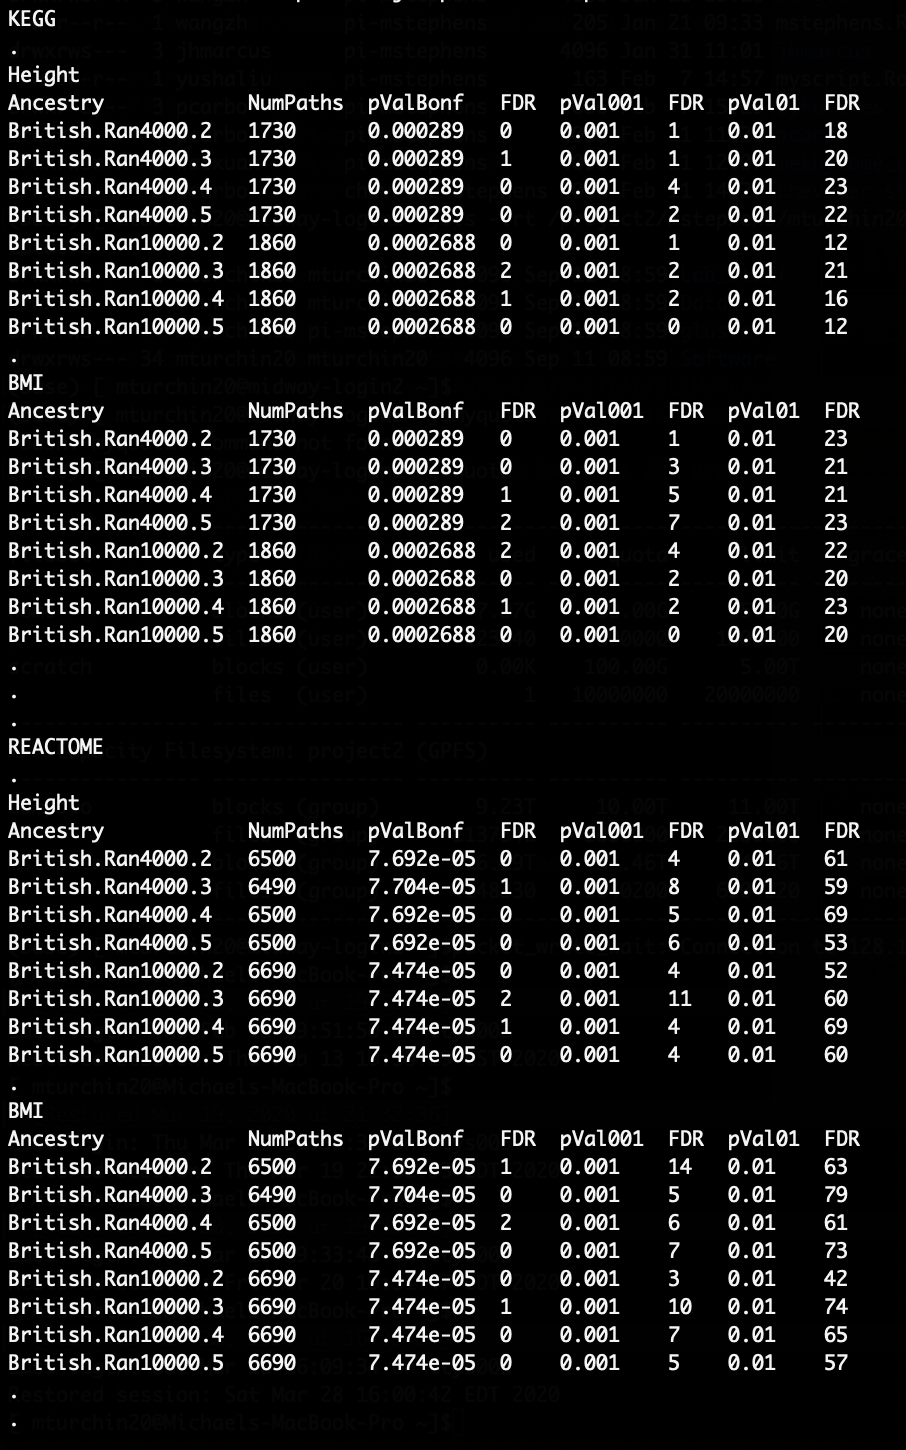
\includegraphics[scale=1.5]{Images/Supp/InterPath_Supp_Figure_FDRs_BritReps_vs1.png}
%\caption[TBD]{\textbf{TBD}. }
%\label{InterPath-Supp-Figure-BritReps-FDRs}
%\end{figure}
%\clearpage




\begin{table}[ht]
\centering
\begin{tabular}{cccc}
  \hline
\textbf{Proteasome} & \textbf{SNP} & \textbf{REACTOME} & \textbf{SNP} \\
\textbf{Gene Family} & \textbf{Counts} & \textbf{Pathways} & \textbf{Counts} \\
  \hline
PSMA & 17 & Activation of NF-KappaB in B Cells & 465 \\
PSMB & 74 & Antigen Processing Cross Presentation & 850 \\
PSMC & 20 & Assembly of the Pre-Replicative Complex & 331 \\
PSMD & 62 & Cell Cycle Checkpoints & 670 \\
PSME & 15 & Cell Cycle & 2459 \\
PSMF & 16 & Cell Cycle Mitotic & 1906 \\
 & & Downstream Signaling Events of the B Cell Receptor & 745 \\
 & & HIV Infection & 1346 \\
 & & Host Interactions of HIV Factors & 963 \\
 & & M G1 Transition & 458 \\
 & & Regulation of Apoptosis & 564 \\
  \hline
\end{tabular}
\end{table}
\clearpage

%\begin{landscape}
\begin{table}[ht]
\resizebox{\textwidth}{!}{
%\tiny
\centering
\hspace*{-3.5cm}
\setlength{\tabcolsep}{1em}
\begin{tabular}{|cc|cccc|}
  \hline
\textbf{Gene Family} & \textbf{SNPs} & \textbf{REACTOME Pathway} & \textbf{SNPs} & \textbf{REACTOME Pathway} & \textbf{SNPs} \\
  \hline
PSMA & 17 & Activation of NF-KappaB in B Cells & 465 & Downstream Signaling Events of the B Cell Receptor & 745 \\
PSMB & 74 & Antigen Processing Cross Presentation & 850 & HIV Infection & 1346 \\
PSMC & 20 & Assembly of the Pre-Replicative Complex & 331 & Host Interactions of HIV Factors & 963  \\
PSMD & 62 & Cell Cycle Checkpoints & 670 & M G1 Transition & 458 \\
PSME & 15 & Cell Cycle & 2459 & Regulation of Apoptosis & 564 \\
PSMF & 16 & Cell Cycle Mitotic & 1906 & & \\
  \hline
%\end{tabular}
\end{tabular}}
\end{table}
\clearpage
%\end{landscape}

[1] "Activation of NF-KappaB in B Cells"     
[2] "Antigen Processing Cross Presentation"  
[3] "Assembly of the Pre-Replicative Complex"
[4] "Cell Cycle Checkpoints"                 
[5] "Cell Cycle"                             
[6] "Cell Cycle Mitotic"                     
 [1] "Activation of NF-KappaB in B Cells"                
 [2] "Antigen Processing Cross Presentation"             
 [3] "Assembly of the Pre-Replicative Complex"           
 [4] "Cell Cycle Checkpoints"                            
 [5] "Cell Cycle"                                        
 [6] "Cell Cycle Mitotic"                                
 [7] "Downstream Signaling Events of the B Cell Receptor"
 [8] "HIV Infection"                                     
 [9] "Host Interactions of HIV Factors"                  
[10] "M G1 Transition"                                   
[11] "Regulation of Apoptosis"                           

\clearpage


\begin{table}[ht]
\centering
\hspace*{0cm}
\begin{tabular}{cc}
  \hline
\textbf{Subgroup} & \textbf{Average Nucleotide} \\
 & \textbf{Divergence per Site} \\
  \hline
African & 0.302 \\
British.Ran4000 & 0.199 \\
Caribbean & 0.290 \\
Chinese & 0.308 \\
Indian & 0.216 \\
Pakistani & 0.216 \\
  \hline
\end{tabular}
\end{table}
\clearpage



\end{document}

